%; whizzy paragraph -pdf xpdf -latex ./whizzypdfptex.sh
%; whizzy-paragraph "^\\\\begin{frame}"
% latex beamer presentation.
% platex, latex-beamer でコンパイルすることを想定。 

%     Tokyo Debian Meeting resources
%     Copyright (C) 2011 Junichi Uekawa
%     Copyright (C) 2011 Nobuhiro Iwamatsu

%     This program is free software; you can redistribute it and/or modify
%     it under the terms of the GNU General Public License as published by
%     the Free Software Foundation; either version 2 of the License, or
%     (at your option) any later version.

%     This program is distributed in the hope that it will be useful,
%     but WITHOUT ANY WARRANTY; without even the implied warreanty of
%     MERCHANTABILITY or FITNESS FOR A PARTICULAR PURPOSE.  See the
%     GNU General Public License for more details.

%     You should have received a copy of the GNU General Public License
%     along with this program; if not, write to the Free Software
%     Foundation, Inc., 51 Franklin St, Fifth Floor, Boston, MA  02110-1301 USA

\documentclass[cjk,dvipdfmx,12pt]{beamer}
\usetheme{Tokyo}
\usepackage{monthlypresentation}

%  preview (shell-command (concat "evince " (replace-regexp-in-string "tex$" "pdf"(buffer-file-name)) "&")) 
%  presentation (shell-command (concat "xpdf -fullscreen " (replace-regexp-in-string "tex$" "pdf"(buffer-file-name)) "&"))
%  presentation (shell-command (concat "evince " (replace-regexp-in-string "tex$" "pdf"(buffer-file-name)) "&"))

%http://www.naney.org/diki/dk/hyperref.html
%日本語EUC系環境の時
\AtBeginDvi{\special{pdf:tounicode EUC-UCS2}}
%シフトJIS系環境の時
%\AtBeginDvi{\special{pdf:tounicode 90ms-RKSJ-UCS2}}

\title{東京エリアDebian勉強会}
\subtitle{第79回 2011年8月度}
\author{岩松 信洋 iwamatsu@debian.org\\IRC nick: iwamatsu}
\date{2011年8月20日}
\logo{
\includegraphics[width=8cm]{image200607/openlogo-light.eps}}

\begin{document}

\frame{\titlepage{}}


\begin{frame}{設営準備にご協力ください。}
宴会場所を誰か探してください。
\end{frame}


\section{}
\begin{frame}
 \frametitle{Agenda}
\begin{minipage}[t]{0.45\hsize}
  \begin{itemize}
  \item 注意事項
	\begin{itemize}
	 \item 飲酒禁止
	 \item 宗教禁止
	 \item 営利活動禁止
	\end{itemize}
   \item 最近あったDebian関連のイベント報告
	\begin{itemize}
	 \item 第78回 東京エリア Debian勉強会
	\end{itemize}
 \end{itemize}
\end{minipage} 
\begin{minipage}[t]{0.45\hsize}
 \begin{itemize}
   \item はじめてのapt\\
    %日常運用からソースビルドまで説明します
   \item パッケージ作成AtoZ 作りながらのQ\&A\\
    %パッケージを作りながら、識者にいろいろ助言をもらいます。
   \item パッケージを作ったら Sponsor Upload\\
    %Debian パッケージのアップロード方法の一つである Sponsor Upload について説明します。
   \item Debconf 11 レポート\\
    %先月末に行われた Debconf 11 のレポートを行います。
  \end{itemize}
\end{minipage}
\end{frame}

\begin{frame}
 \frametitle{前回}
\begin{minipage}[t]{0.45\hsize}
  \begin{itemize}
  \item 注意事項
	\begin{itemize}
	 \item 飲食禁止
	 \item 宗教禁止
	 \item 営利活動禁止
	\end{itemize}
  \end{itemize}
\end{minipage}
\begin{minipage}[t]{0.45\hsize}
 \begin{itemize}
  \item 最近あったDebian関連のイベント報告
  \begin{itemize}
   \item Debconf11 in ボスニア
  \end{itemize}
 \end{itemize}
\end{minipage}
\end{frame}


\emtext{イベント報告}

\emtext{DWN quiz}

\section{DWN quiz}
\begin{frame}{Debian 常識クイズ}

Debian の常識、もちろん知ってますよね?
知らないなんて恥ずかしくて、知らないとは言えないあんなことやこんなこと、
みんなで確認してみましょう。

今回の出題範囲は\url{debian-devel-announce@lists.debian.org} に投稿された
内容とDebian Project Newsからです。

\end{frame}

\subsection{問題}
%; whizzy-master ../debianmeetingresume201101.tex
% $B0J>e$N@_Dj$r$7$F$$$k$?$a!"$3$N%U%!%$%k$G(B M-x whizzytex $B$9$k$H!"(Bwhizzytex$B$,MxMQ$G$-$^$9!#(B
%
% $B$A$J$_$K!"%/%$%:$OJL%V%i%s%A$G:n@.$7!"$N$A$K%^!<%8$7$^$9!#5U$K%^!<%8$7(B
% $B$J$$$h$&$K$7$^$7$g$&!#(B
% (shell-command "git checkout quiz-prepare")

\santaku
{alioth.debian.org$B$,(B2$BBf$KJ,$+$l$^$7$?!#$=$N%5!<%PL>$O!)(B}
{vasks.debian.org $B$H(B wagner.debian.org}
{volks.debian.org $B$H(B don.debian.org}
{dennys.debian.org $B$H(B gusto.debian.org}
{A}
{$B$[$+$O%U%!%_%l%9$NL>A0(B}

\santaku
{$B8=:_9T$o$l$F$$$k(BPerl transition $B$N(BPerl$B%P!<%8%g%s$O!)(B}
{5.12}
{5.13}
{5.14}
{A}
{5.14$B$O$^$@(Bexperimental$B$G$9!#(B}

\santaku
{$B%W%i%$%^%j%_%i!<%5!<%P$,?7$7$/DI2C$5$l$?9q$O!)(B}
{$B%A%e%K%8%"(B}
{$BCf9q(B}
{$B%^%@%,%9%+%k(B}
{B}
{$B%A%e%K%8%"$H%^%@%+%9%+%k$O%_%i!<!#%W%i%$%^%j$G$O$J$$!#(B}


\emtext{prework}

{\footnotesize
 %; whizzy-master ../debianmeetingresume201108.tex
% 以上の設定をしているため、このファイルで M-x whizzytex すると、
% whizzytexが利用できます

\begin{prework}{ 鈴木崇文 }

aptのリポジトリ作成ってどうやるのでしょうか。
ググったらなんかページが出てきてわかりそうですが、やったことないので書きました。
あと、以前誰かが話していたaptのキャッシュサーバーって最近の動向はどうなのでしょうか。

\end{prework}

\begin{prework}{ キタハラ }

Debian固有のものだと、今のところないですね。
1コマンド(又はGUI操作)でUSBメモリにLive環境を作るツールとか?
(探すとあったりして…、調べていません。)

\end{prework}

\begin{prework}{ やまだ }

今後調べたい(解説歓迎)
\begin{itemize}
\item libapt-pkg-perl/python-aptなどのパッケージデータベースAPI
\item debhelper8(簡単になったが奥行きがさらに増した、ような…)
\item *.d.oなサイトを改良したくなったらどうすればいいか
\end{itemize}

緩募
\begin{itemize}
\item apt-buildの./configureの引数なども即いじれる版
\item apt-get changelog風の入れてないマニュアル等を読むツール
\end{itemize}

\end{prework}

\begin{prework}{ koedoyoshida }

dpkg -i(apt-get installも同様)がエラーになったときの原因追及で困ったことがあったので、そのようなときの調査法を知りたい。
\url{http://www.flcl.org/~takasugi/tdiary-org/?date=20061023}
に同現象があったのでとりあえずワークアラウンドは分かりましたが...

\end{prework}

\begin{prework}{ dictoss(杉本 典充) }

debootstrapのおもしろい使い方ってあるのかなぁ。(amd64上でi386環境が必要、常用環境とテスト環境の分離、くらいしか使ったことないです。)
\end{prework}

\begin{prework}{ 上川純一 }
とくになし。

\end{prework}

\begin{prework}{ Osamu MATSUMOTO }

ユーザーとしては特に困ってないっす。aptitudeでしかできない事ってあるのかわかりません。開発者ツールまだまだ勉強中。
\end{prework}

\begin{prework}{ なかおけいすけ }

\begin{itemize}
\item aptのオプションの解説

apt-get update, upgrade, install, remove, clean 位しか使ってないのでその他のオプションについて

\item 推奨パッケージもインストールしてくれるオプション

これはきっとある

\item apt.confの解説

debianのページを見ていると、時々apt.confを修正してみたいな記述があるけれども、何をやっているのか、何ができるのか、解説が欲しい。

\item apt-getとaptitudeの違い
\end{itemize}

\end{prework}

\begin{prework}{ やまねひでき }

debootstrapでxzがサポートされていると良いのかも。
\end{prework}

\begin{prework}{ 岩松 信洋 }

ぱっとは思いつかないです。
\end{prework}

\begin{prework}{ 吉野(yy\_y\_ja\_jp) }

こんにちは。
\end{prework}

\begin{prework}{ yamamoto }

最近は apt-get autoremove で、既に削除されたパッケージの、依存関係解決のために入れられたパッケージがごっそり削除できますが、apt-get build-dep ホゲホゲで入れられたパッケージも同じようにビルド終了後に消せるといいよね。
\end{prework}

\begin{prework}{ taitioooo }

課題は未定ですが。
debianでkaresansuiが使えるようになるといいですね〜

あ、やればいいのか!
\end{prework}

}

\emtext{はじめてのapt}
\emtext{パッケージ作成AtoZ 作りながらのQ\&A}

\emtext{パッケージを作ったら Sponsor Upload}

\begin{frame}{はじめに}

\begin{itemize}
\item Debian にパッケージをアップロードする場合、誰でもアップロードできるわけではなく
限られた人しかアップロードできない。

\item アップロードできるのはDebian Developer(以下、DD)とDebian Maintainer(以下、DM)
だけ。また、DM はアップロードする際に制限がある。

\end{itemize}


%\begin{figure}[ht]
 \begin{center}
  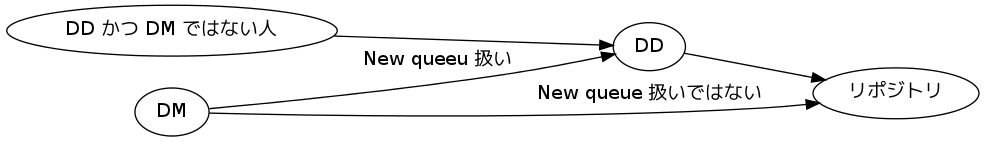
\includegraphics[width=1.0\hsize]{image201108/sponsor0.png}
 \end{center}
%\label{fig:sponsor0}\caption{パッケージアップロード}
%\end{figure}


\end{frame}

\begin{frame}

\begin{itemize}[<+->]
\item DDではない人が、メンテナンスしているパッケージをアップロード
したい場合には、DD に頼んでアップロードしてもらう必要がある。

\item パッケージを代理でアップロードする人をスポンサー。
\item アップロードする行為をスポンサーアップロード。

\item パッケージメンテナに変わってパッケージをアップロードするので、パッケージに対して
責任が問われる作業。
\item スポンサーはパッケージのチェック等を行ったりパッケージ内容に対して助言をす
る(mentor)。 
\item このパッケージチェックの過程は DD や DMになる場合に優位に働く場合がある、
\end{itemize}

\end{frame}


\begin{frame}{スポンサーアップロードするときに確認する内容}

\begin{itemize}
\item パッケージメンテナに「アップロードして!」と言われてすぐにアップロードできるものではない。 
\item スポンサーはアップロードするパッケージメンテナとパッケージを
確認する必要があります。
\end{itemize}

\end{frame}

\begin{frame}{パッケージをチェックする前のチェック}

スポンサーをするパッケージメンテナの方に以下の内容を確認しています。

\begin{itemize}[<+->]
\item Web of Trust(WOT) に入っているか。
\item DDやDMへの意欲はあるか。
\item Debian 新メンテナーガイドを読んだか。
\item DFSG を読んだか。
\item Debian Policy を読んだか。
\item Debian Reference を読んだか。
\end{itemize}

%これ以外にも、たまに誰もスポンサーする人がいないようなのでスポンサーする場合があります。
\end{frame}

\begin{frame}{パッケージのチェック}

\begin{itemize}[<+->]

\item ライセンスの確認

ソフトウェアのライセンスがDFSGに合致するライセンスか、ライセンスが debian/copyright に書かれているか確認します。
この確認には devscripts パッケージに含まれる licensecheck を使うことが多いです。

\item orig.tar.gz の確認

オリジナルのtarボールと一緒か、オリジナルのソースコードに
変な改変をしていないかを確認します。

\item 最新のパッケージングのルールに合っているかの確認。

例えば、使っているプログラミング言語向けのパッケージングサポートツールが新しくなっていたり、
パッケージングポリシーが決まっている場合があります。できるだけ新しいパッケージングのルールに
合わせるようにします。

\end{itemize}
\end{frame}


\begin{frame}{パッケージのチェック}

\begin{itemize}[<+->]


\item debian/control ファイルの確認

依存関係、パッケージの説明、各セクションの確認を行います。

\item debian/rules の確認

シンプルな構成になっているか、ポリシーに違反していないかの確認。

\item pbuilder を使ったパッケージビルドの確認

pbuilder / cowbuilder /  sbuild を使って、最新unstable ディストリビューションでパッケージがビルドできるか確認します。
lintian によるチェックや、ビルドに必要なパッケージが依存関係から漏れていないか
確認することができます。

\item lintianを使ったポリシーとパッケージングミスの確認

パッケージが Debian ポリシー に準拠しているか簡単に確認するには
lintian\footnote{\url{http://packages.qa.debian.org/l/lintian.html}} を使います。
これはDebian ポリシー の他に Debian パッケージのよくある間違いに関してチェックしてくれます。


\end{itemize}
\end{frame}


\begin{frame}{パッケージのチェック}

\begin{itemize}[<+->]


\item メンテナスクリプト(preinst、postinst、prerm、postrm、コンフィグ)の確認
\item オリジナルの tar ボールとの差分の確認

diff.gz の内容を確認します。
作成されたパッチは上流開発者に送ってあるか、パッチはDEP3
\footnote{\url{http://dep.debian.net/deps/dep3/}}
に対応しているか、確認します。

\item パッケージのインストール、アンインストールの確認

パッケージはできても、インストールできない場合やアンインストールできない場合があります。
またパッケージが動作しない場合もあります。このような問題
がないか確認するために、
piuparts\footnote{\url{http://packages.qa.debian.org/p/piuparts.html}} を使ってインストール、アンインストールのチェックと、実際にインストールしてみて動作するか確認をします。

\end{itemize}
\end{frame}

\begin{frame}{その他}
その他、スポンサーによっては以下のような理由でスポンサーしてくれない場合があるようです。
注意しましょう。

\begin{itemize}

\item スポンサーをUploaderに入れることを要求される場合がある。
\item パッケージング用のツールを要求される場合がある。
\item \url{http://mentors.debian.net} を使わない場合はスポンサーをしない。
\item 自分の知らないプログラミング言語で書かれたパッケージはスポンサーをしない。

\end{itemize}
\end{frame}

\begin{frame}

また、\url{http://wiki.debian.org/SponsorChecklist}
に実際にスポンサーしている人の方針が纏められています。
\end{frame}

\begin{frame}{アップロード}
アップロードには、dput や dupload パッケージを使います。
実装が異なるだけで、基本的な機能は揃っているのでどちらでも使い方は同じです。
\end{frame}

\begin{frame}{まとめ}
以上のようにスポンサーになることはとても大変なので、メンテナの方はさっさとDMかDDになりましょう。
\end{frame}


\emtext{Debconf 11 レポート}

\begin{frame}{開催場所}
\begin{minipage}{0.6\hsize}
\begin{itemize}
\item 開催場所は ボスニア・ヘルツェゴビナのバニャルカ州。
\item 日本から直行便がないので、周辺の国でトランジットしてクロアチア経由で入国。
\item 所要時間は約15時間。
\item バニャルカ州の完全サポート。
\item 今回の参加者は約350名。
\item 日本からは、やまねさん、野島さん、岩松の3人が参加。
\end{itemize}
\end{minipage}
\begin{minipage}{0.35\hsize}
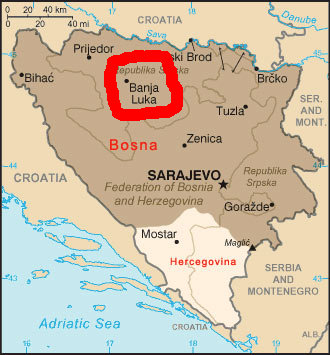
\includegraphics[width=1.4\hsize]{image201108/debconf11_map.jpg}
\end{minipage}
\end{frame}

\begin{frame}{会場}

会場は、バニャ・ルカの施設であるBanski Dvor カルチャーセンターで行われ
た。会場内で使用された施設は以下の通りである。
\begin{center}
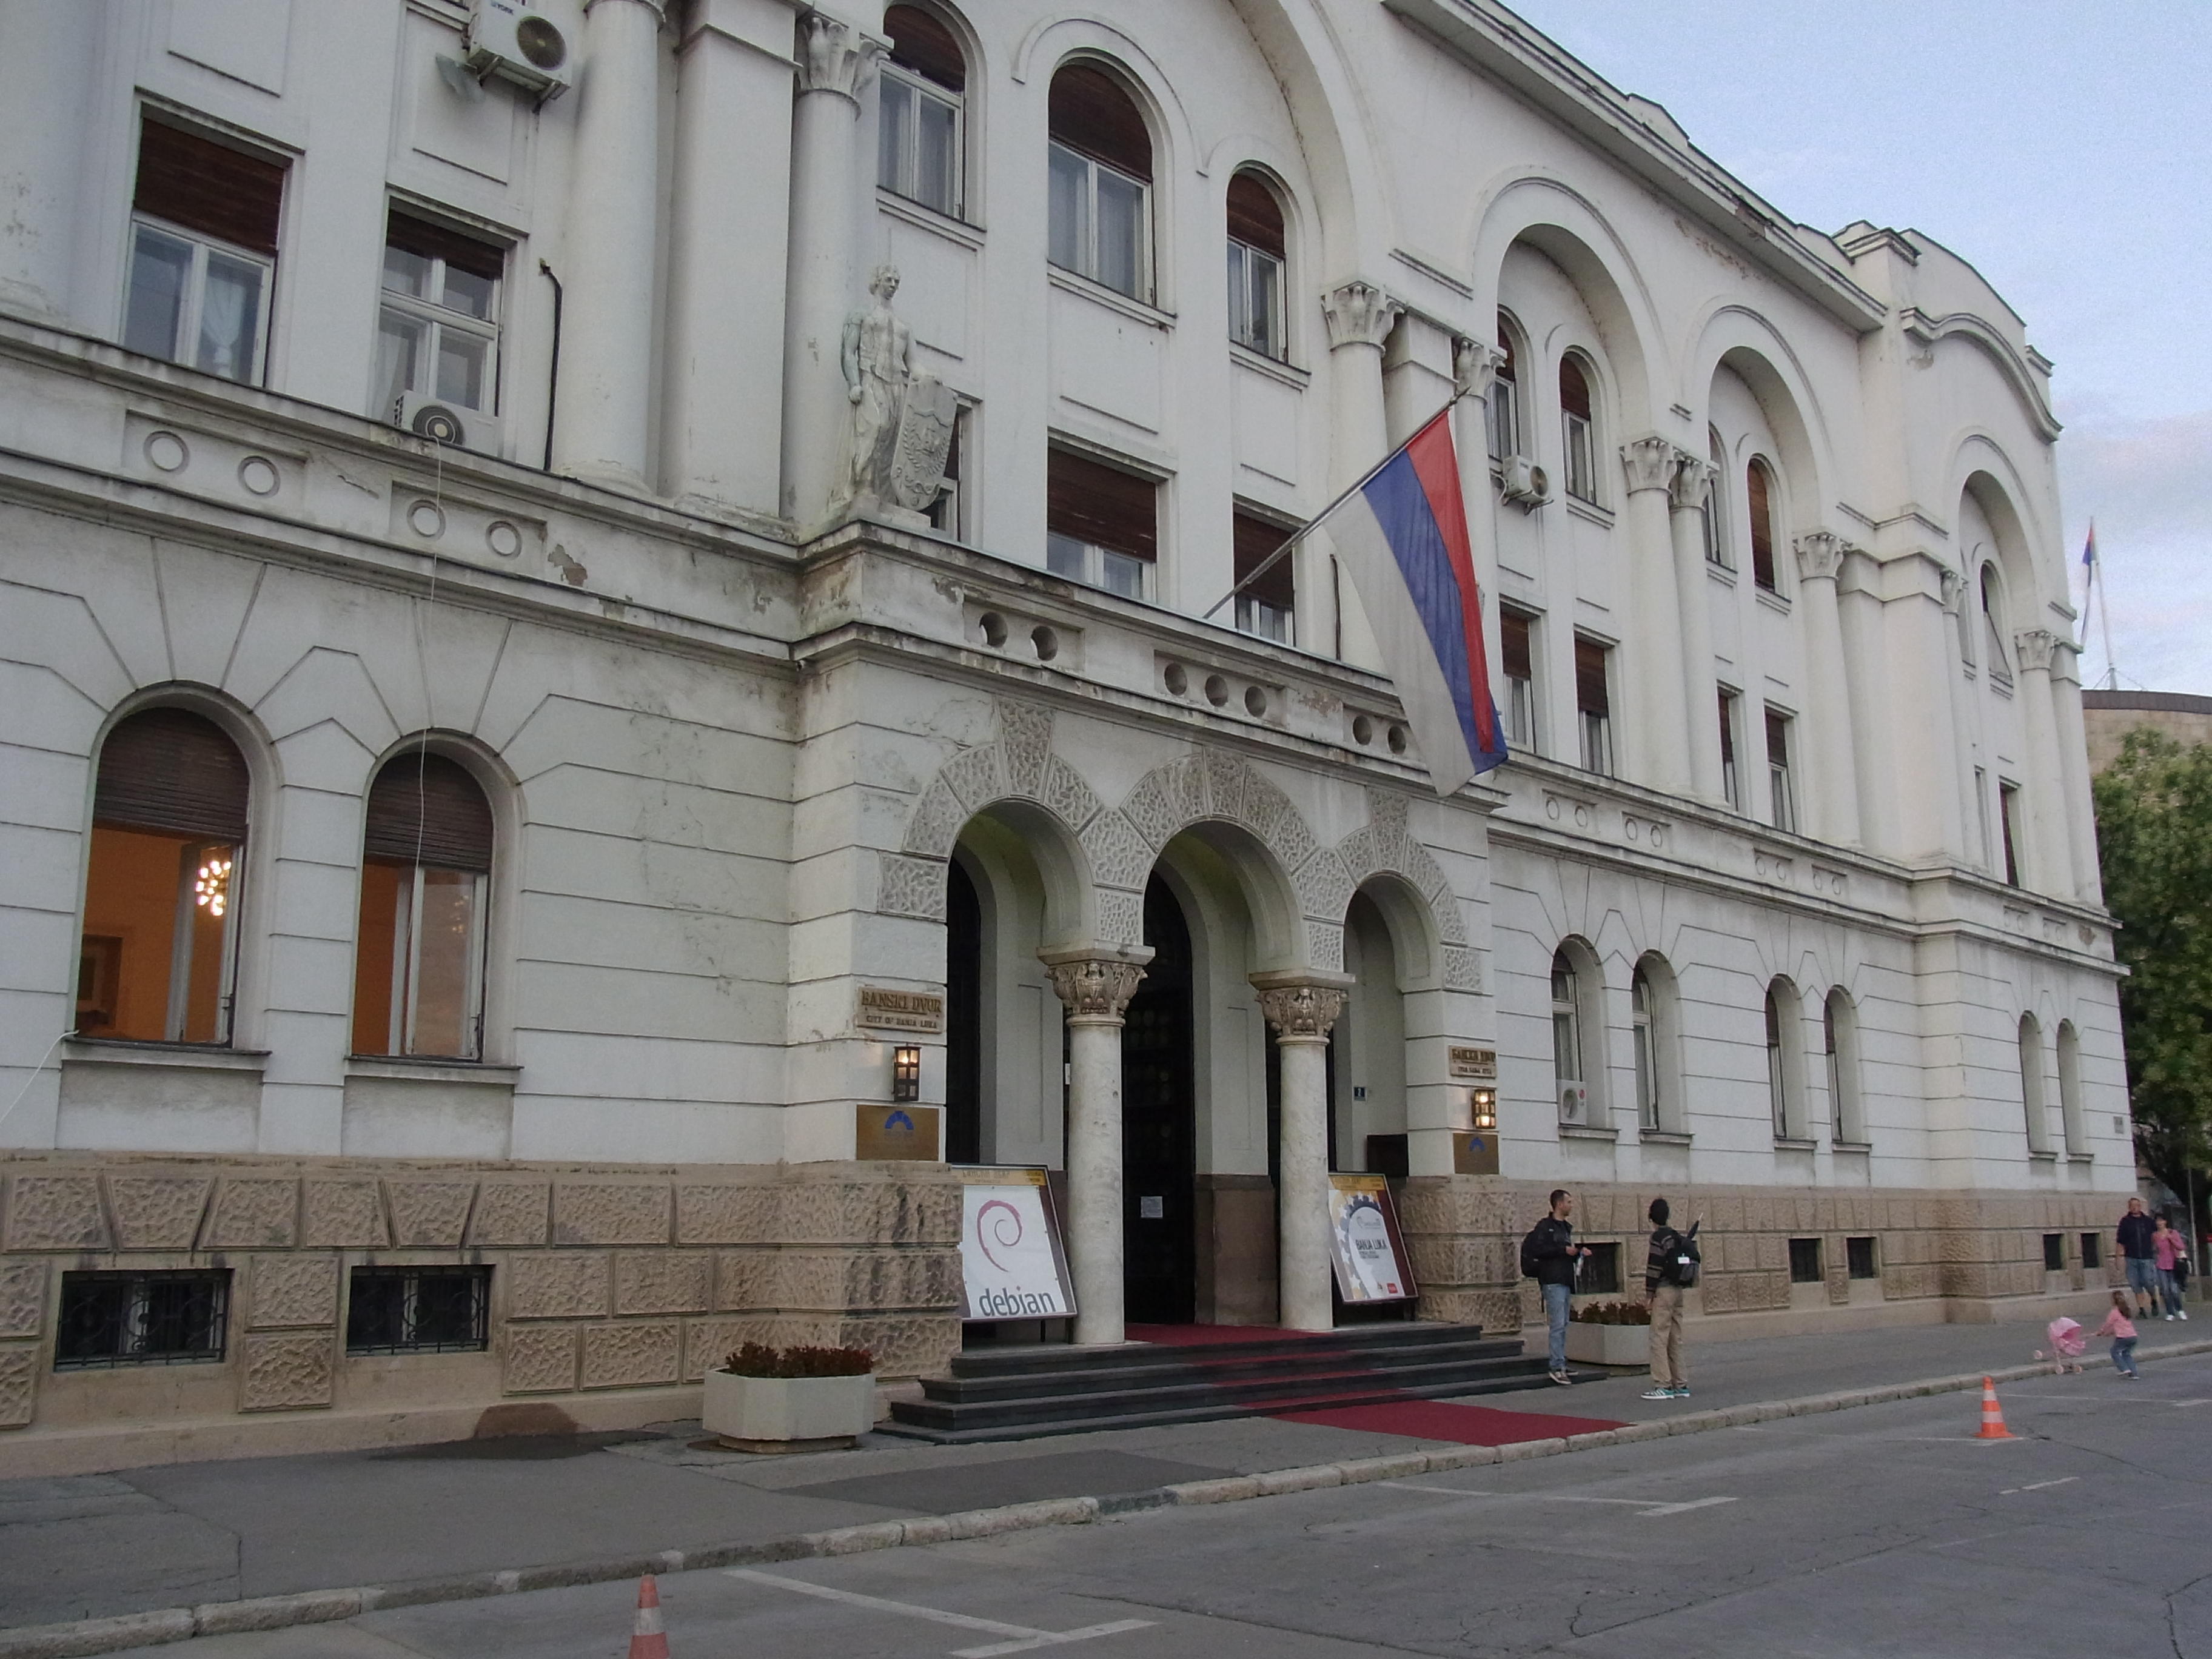
\includegraphics[width=0.8\hsize]{image201108/debconf11_venue1.jpg}
\end{center}
\end{frame}

\begin{frame}{会場の前にある教会}
\begin{center}
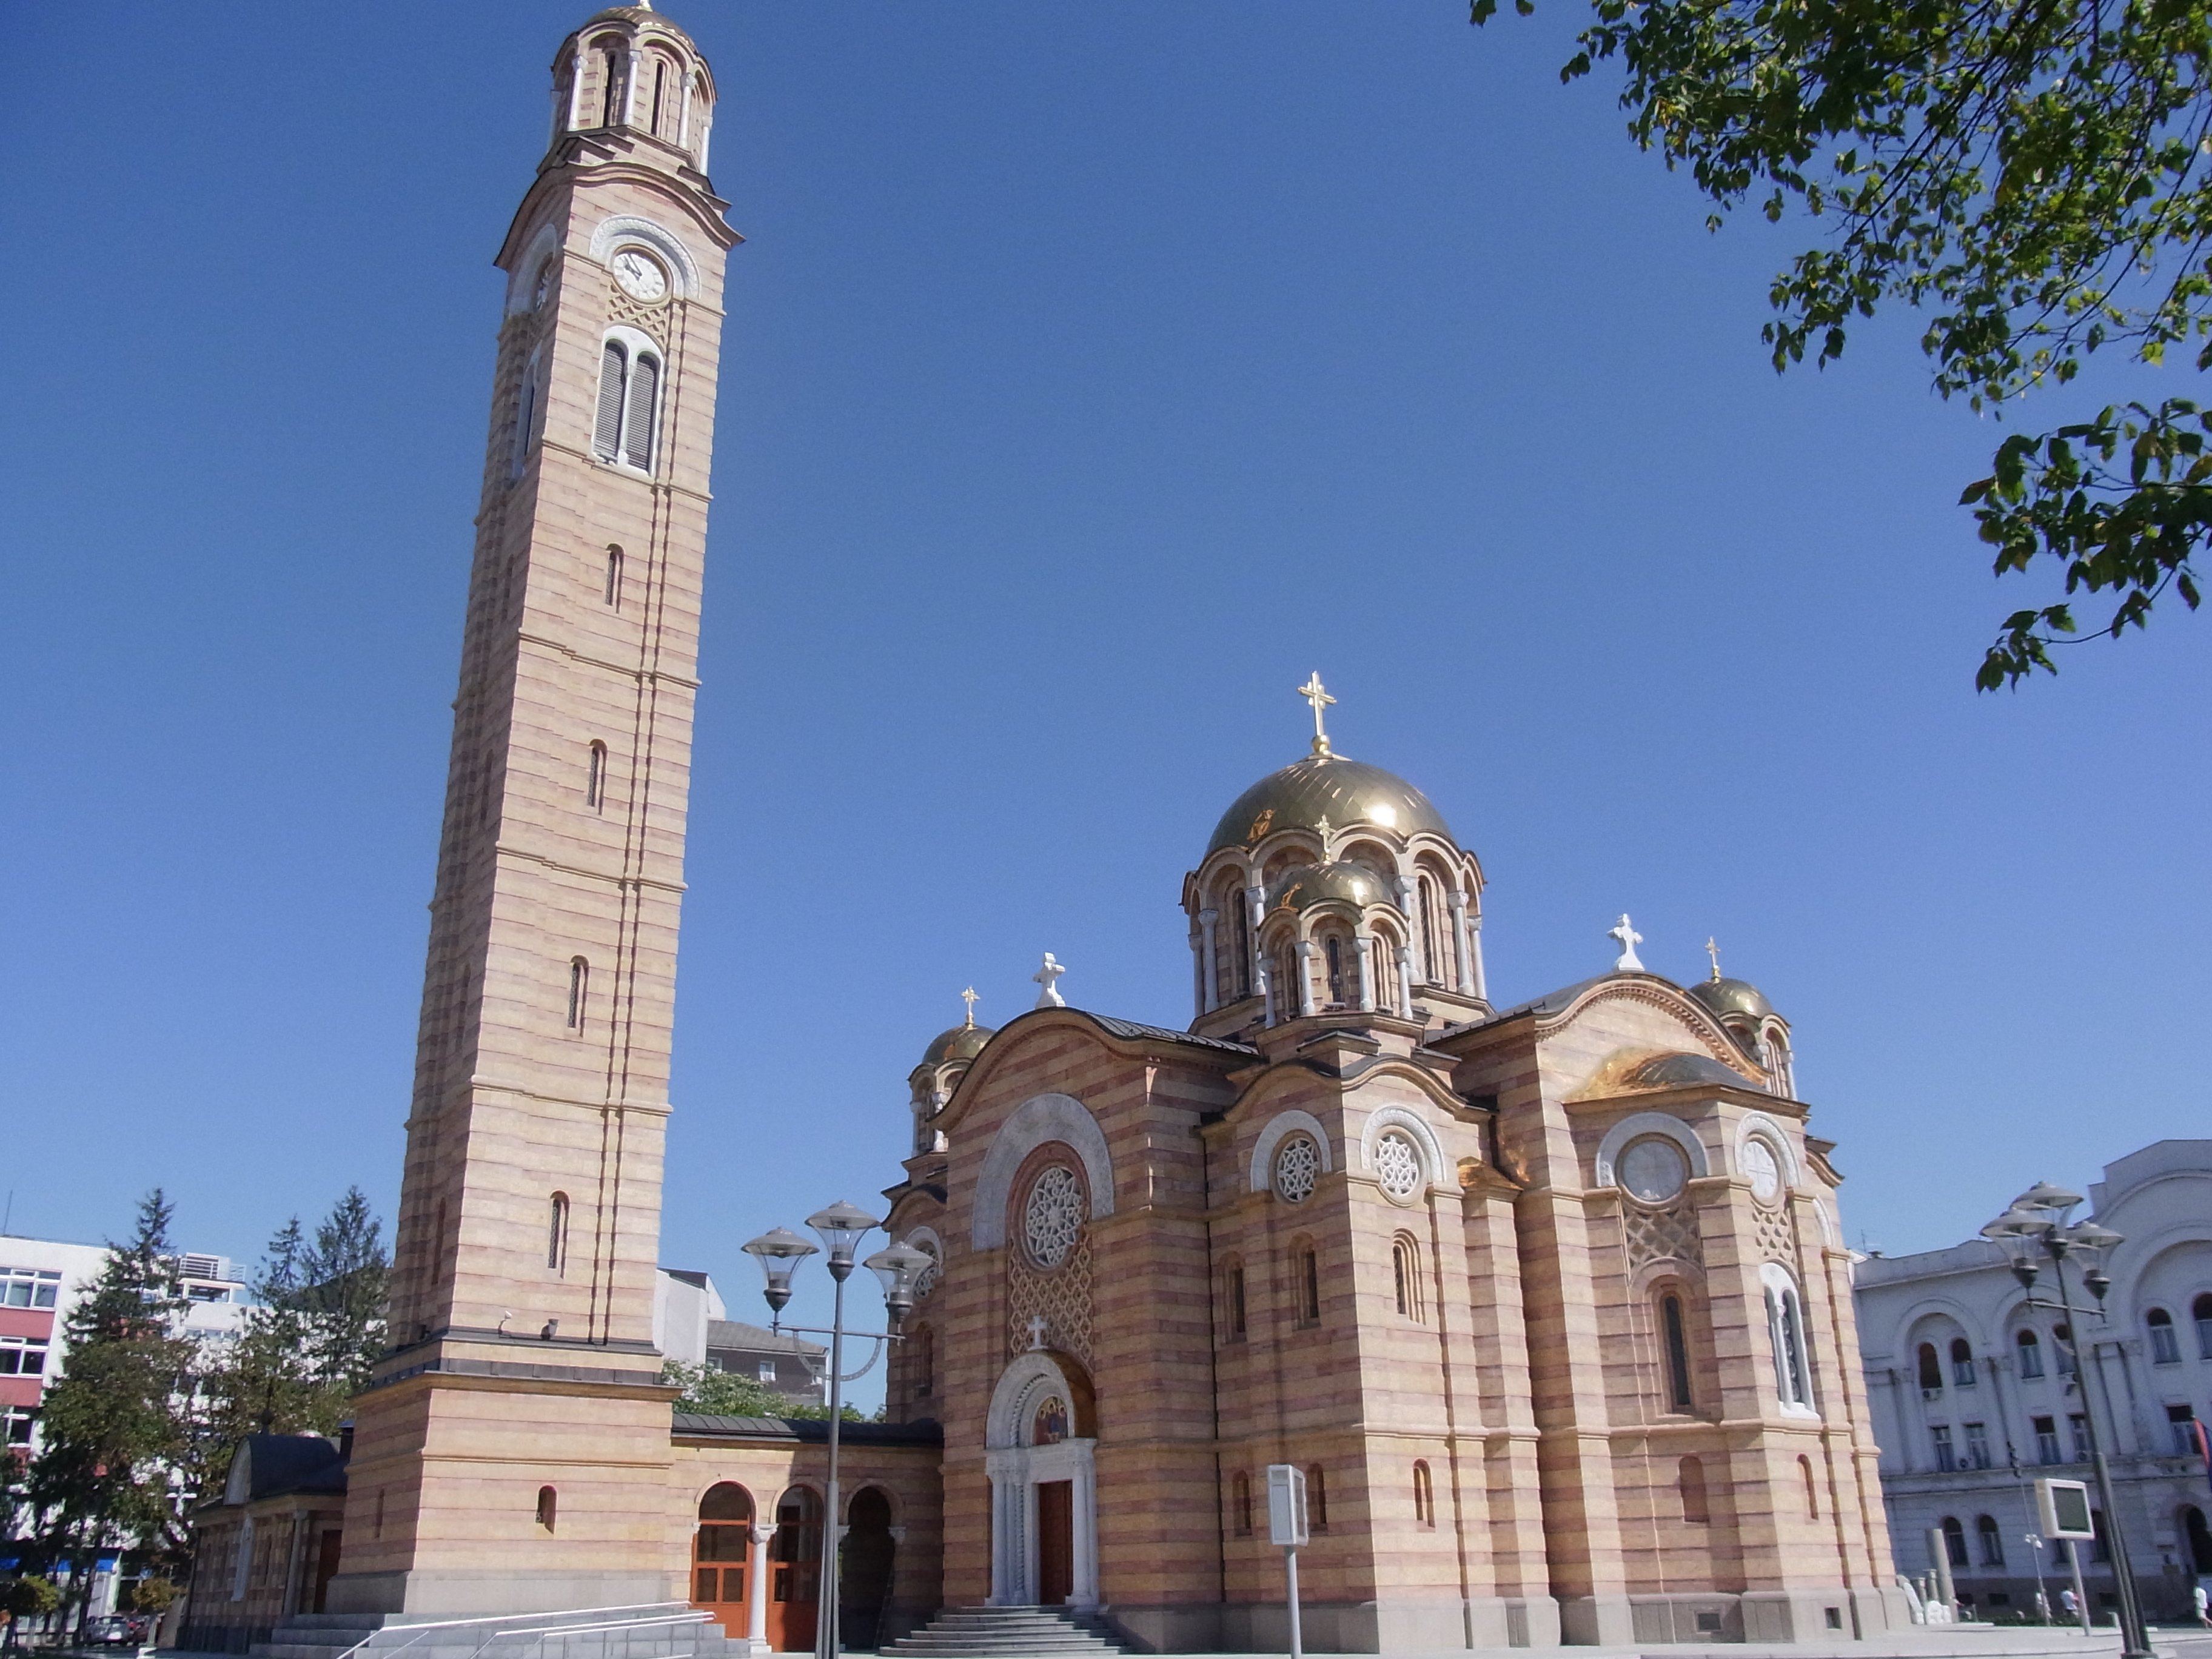
\includegraphics[width=0.8\hsize]{image201108/debconf11_venue2.jpg}
\end{center}
\end{frame}

\begin{frame}{Auditorium} 
メイン用。400人ほど入ることができる。\\
\begin{center}
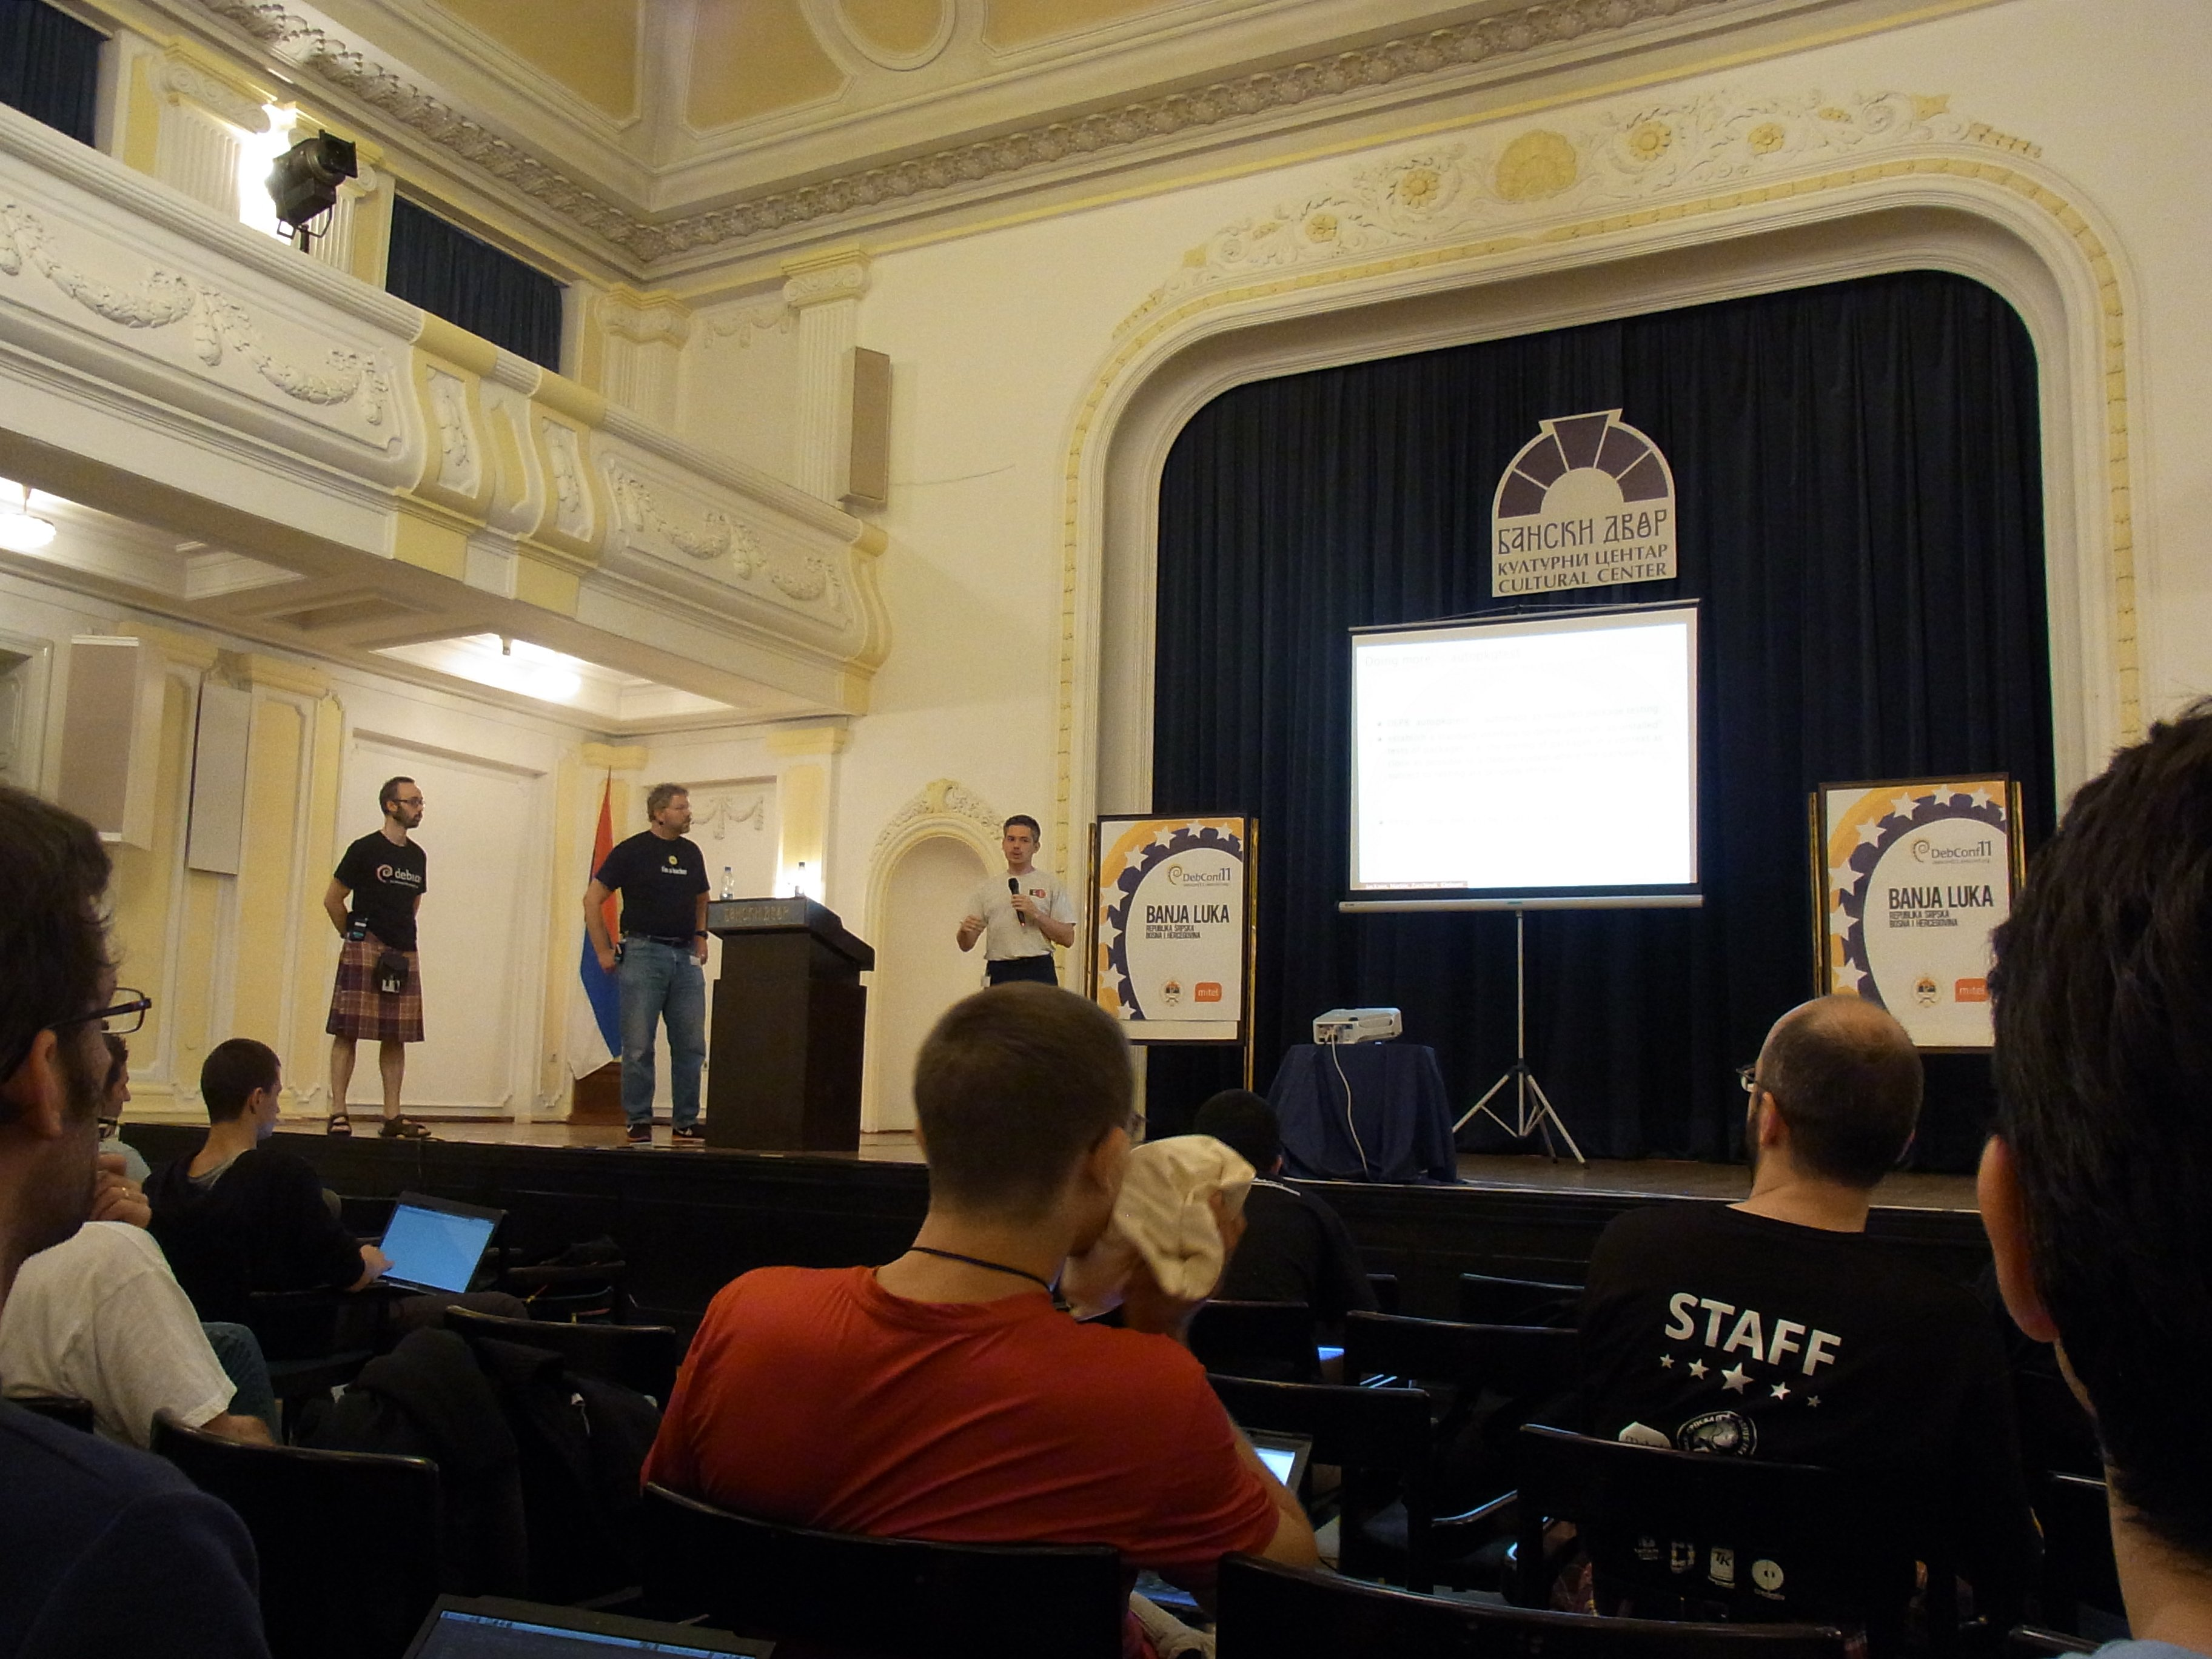
\includegraphics[width=0.9\hsize]{image201108/debconf11_main.jpg}
\end{center}
\end{frame}

\begin{frame}{Round room} 
サブ会場。50人ほど入ることができる。\\
\begin{center}
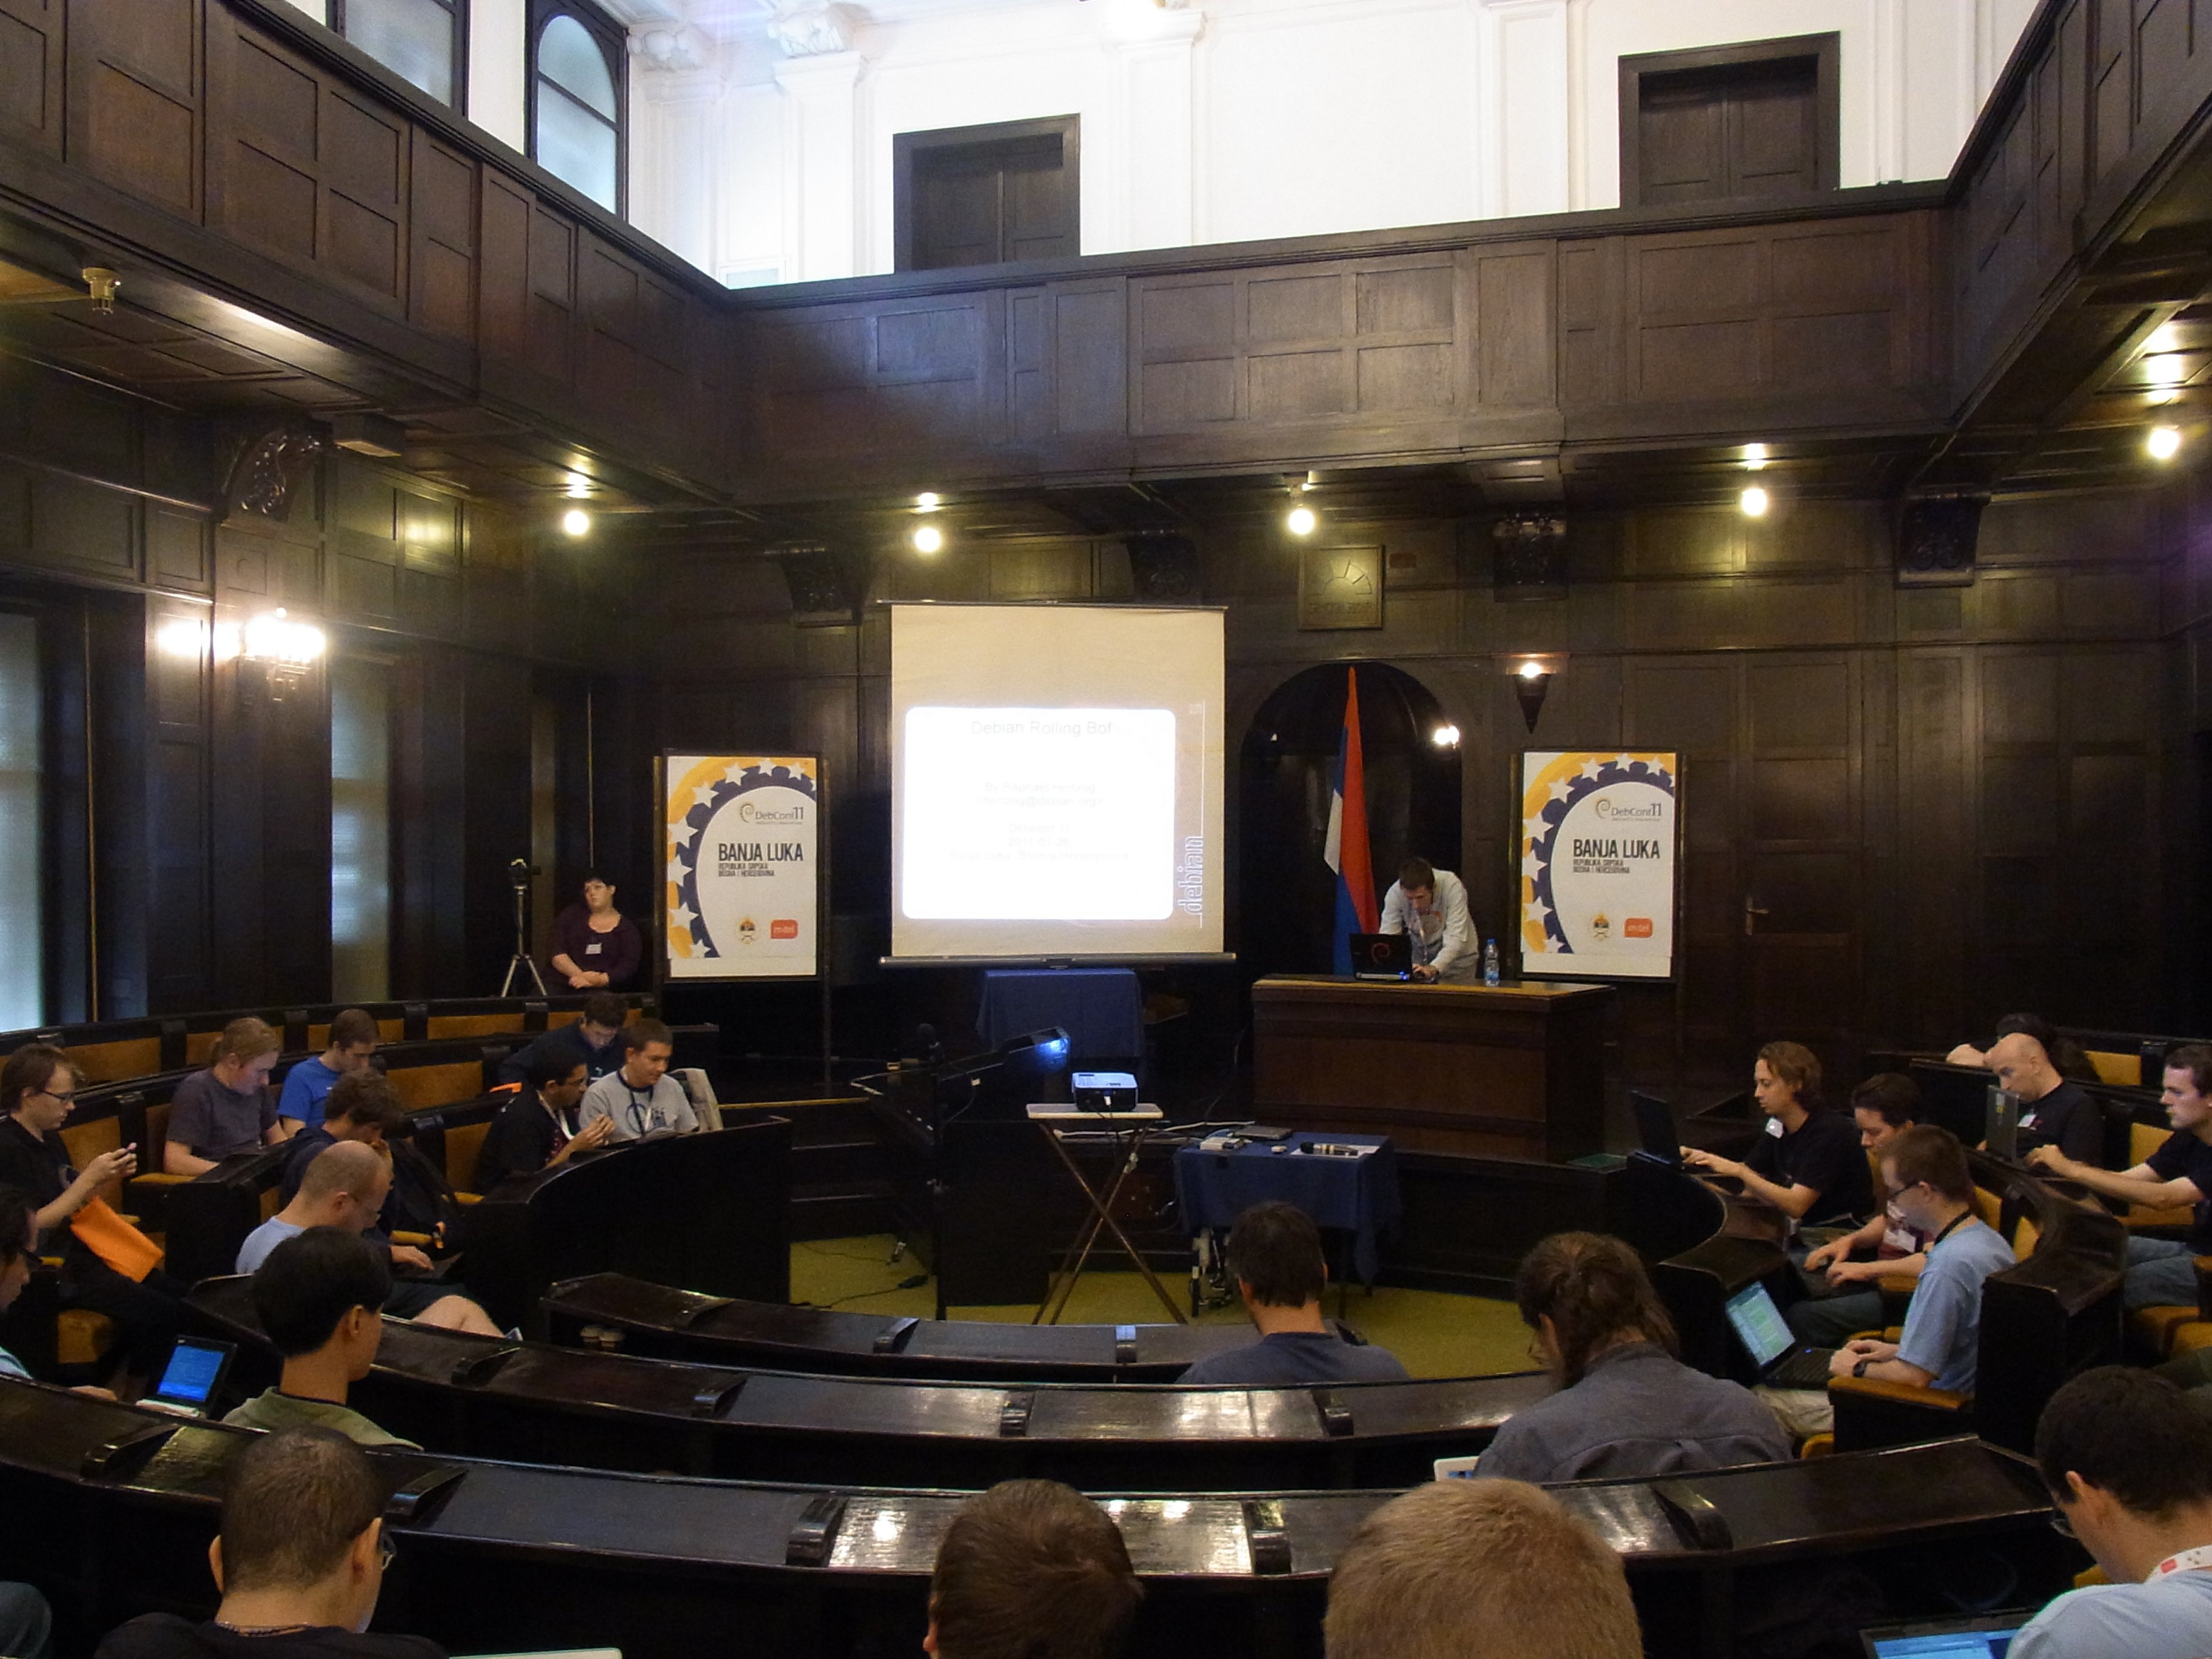
\includegraphics[width=0.9\hsize]{image201108/debconf11_room2.jpg}
\end{center}
\end{frame}

\begin{frame}{meeting room}
BOF 用。30人ほど入ることができる。
\begin{center}
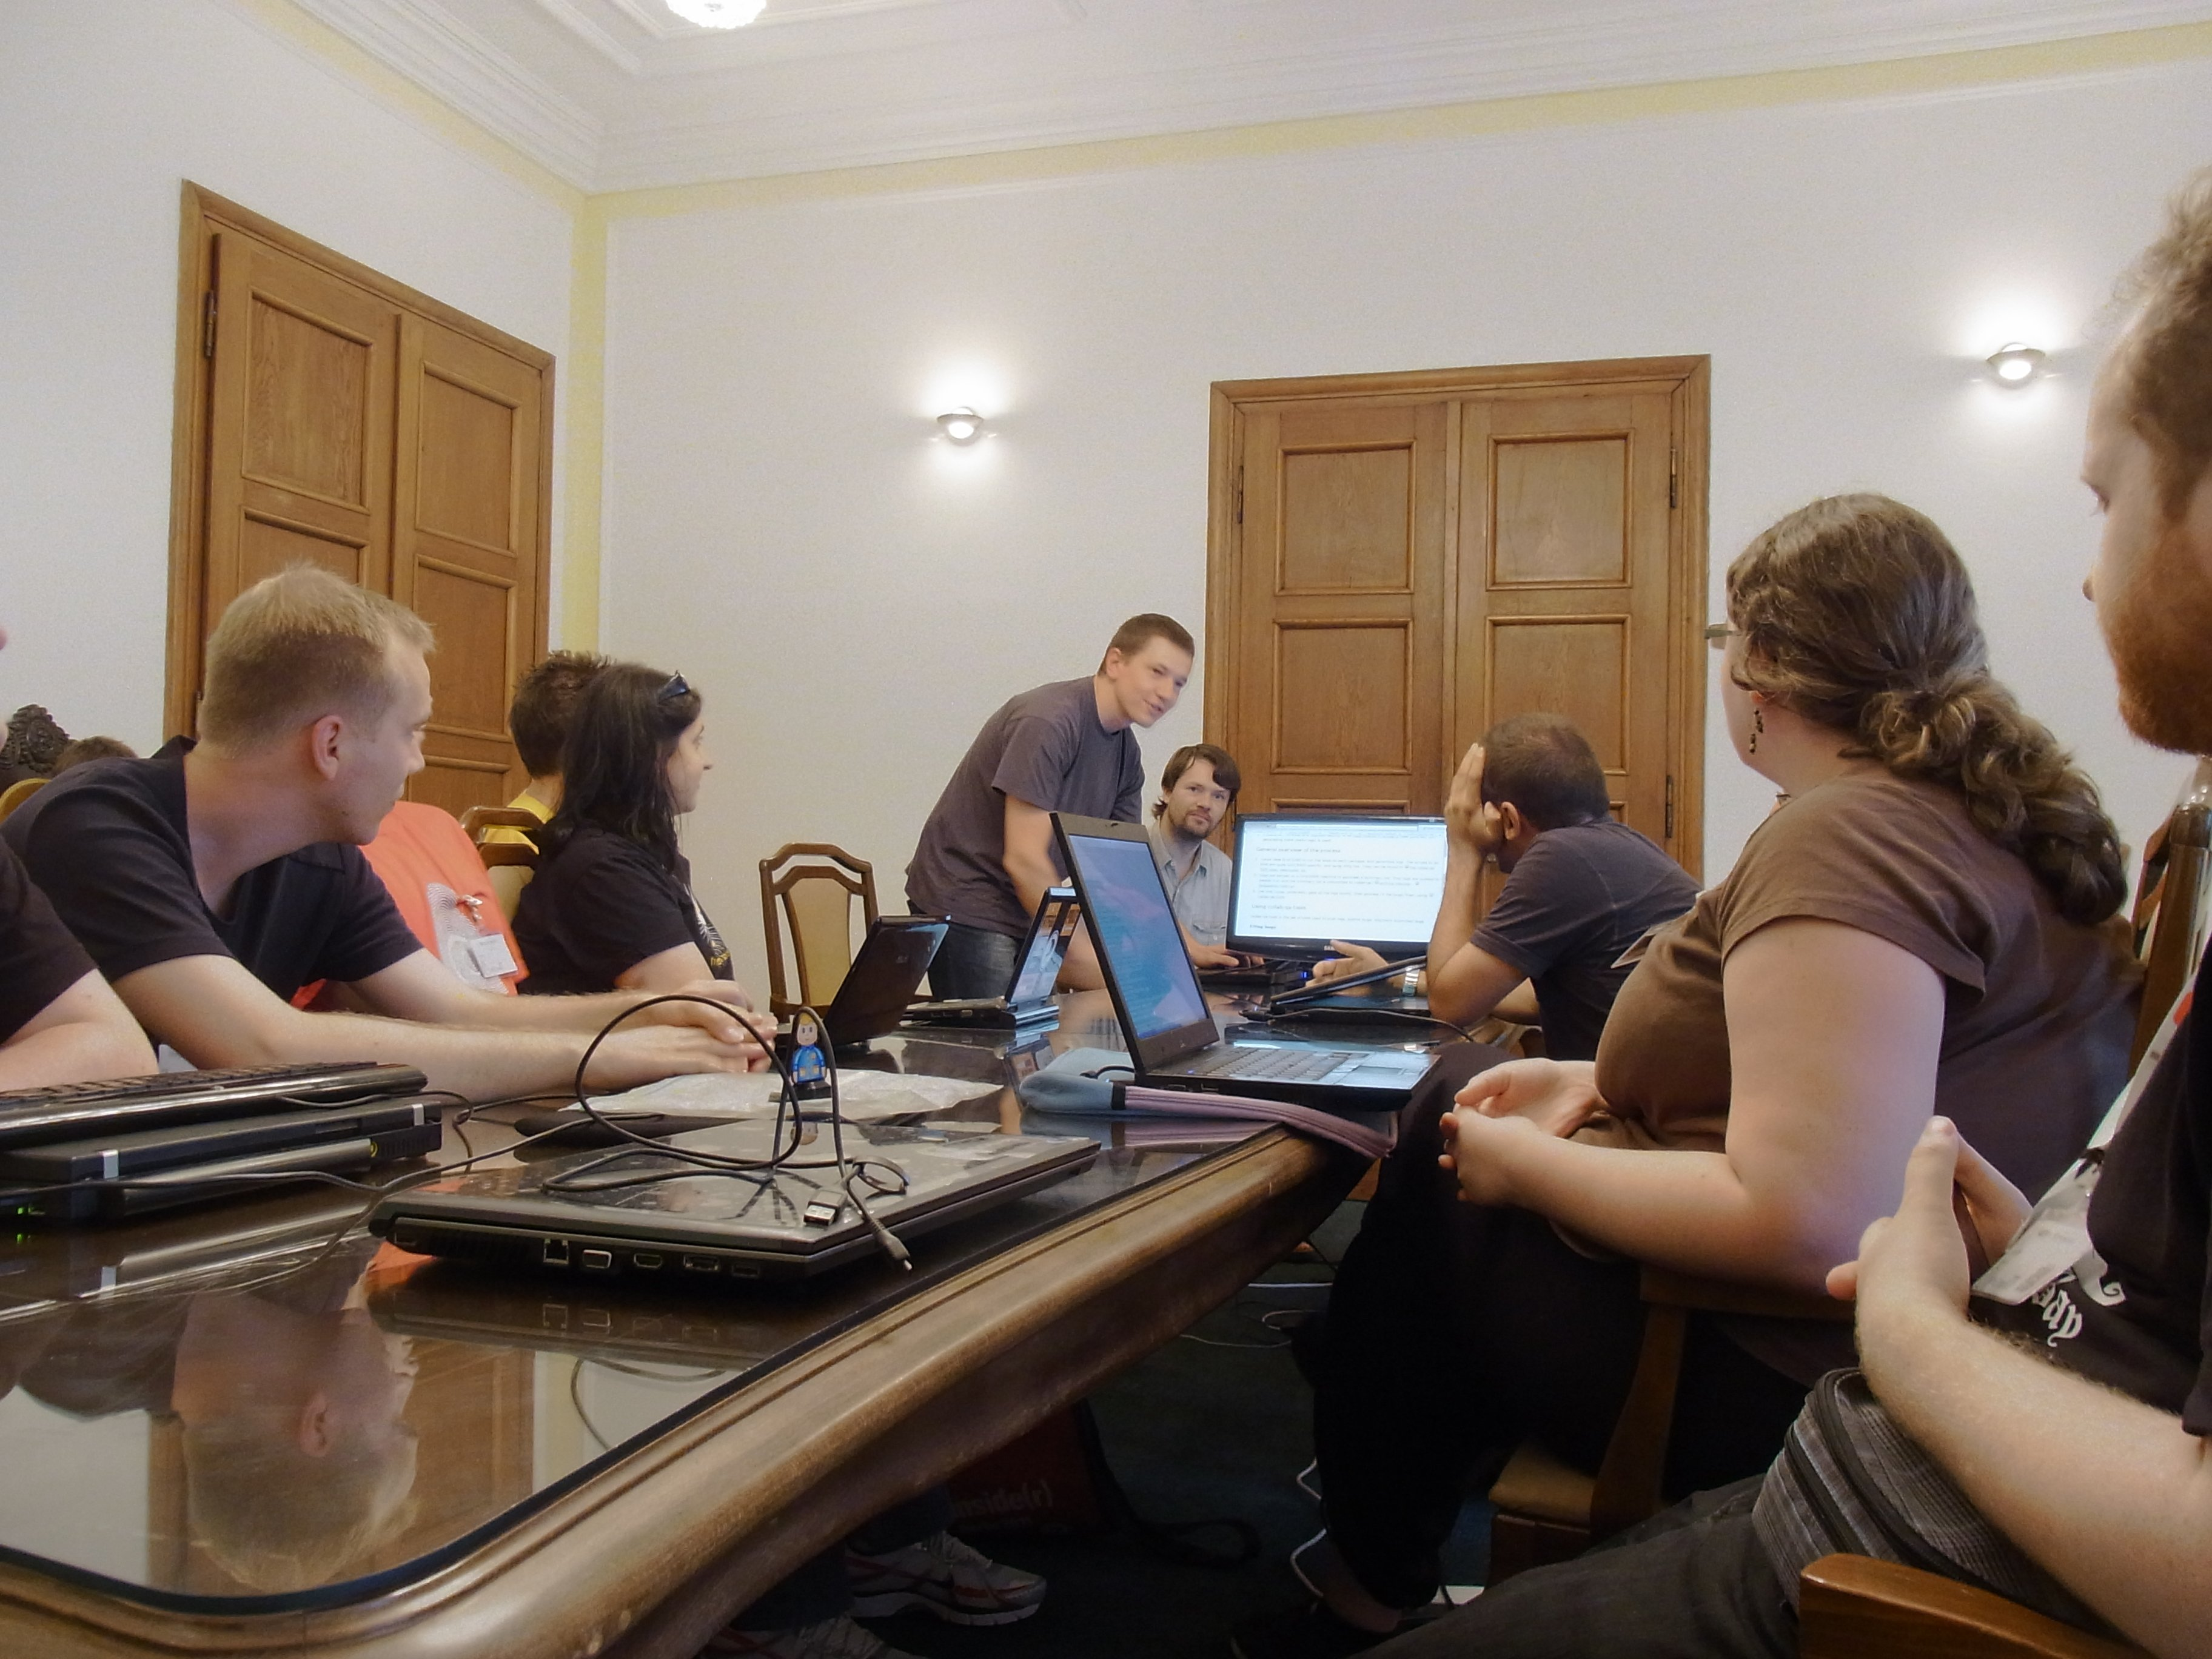
\includegraphics[width=0.9\hsize]{image201108/debconf11_meetingroom.jpg}
\end{center}
\end{frame}

\begin{frame}{Hacklab1}

Hacklab はハック専用の部屋。\\
\begin{center}
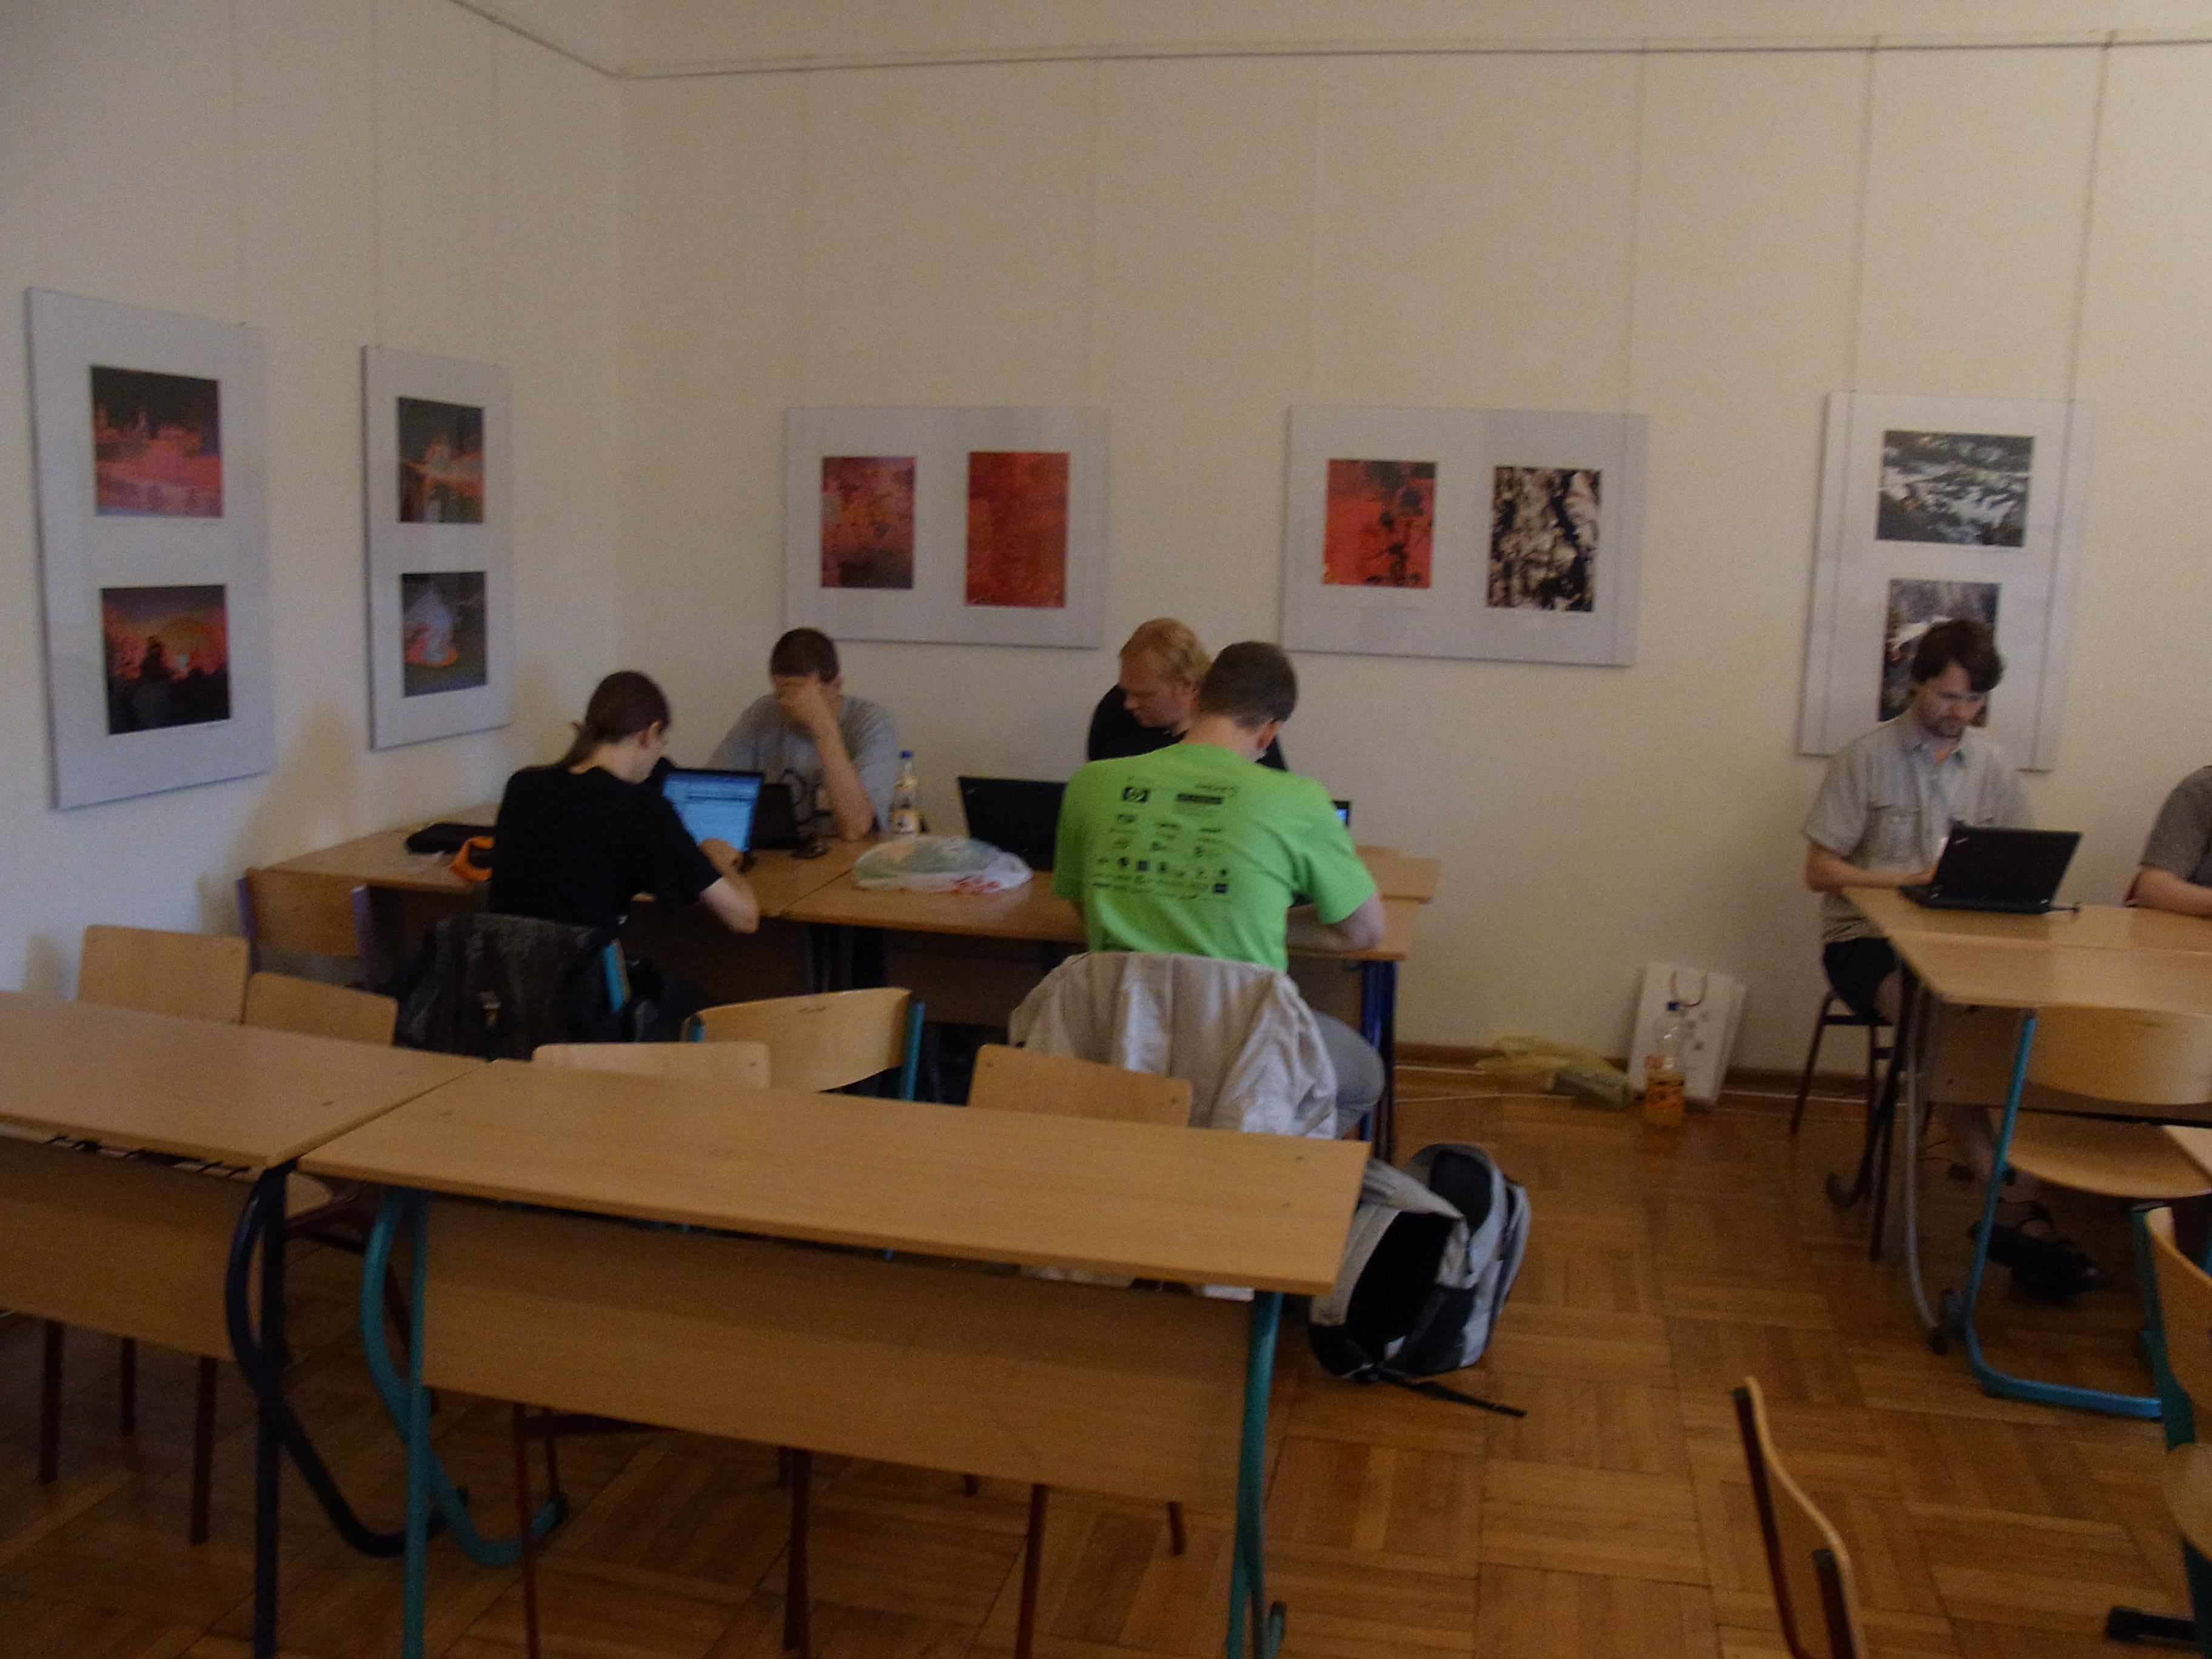
\includegraphics[width=0.8\hsize]{image201108/debconf11_hacklab1.jpg}
\end{center}
\end{frame}

\begin{frame}{Hacklab2}
\begin{center}
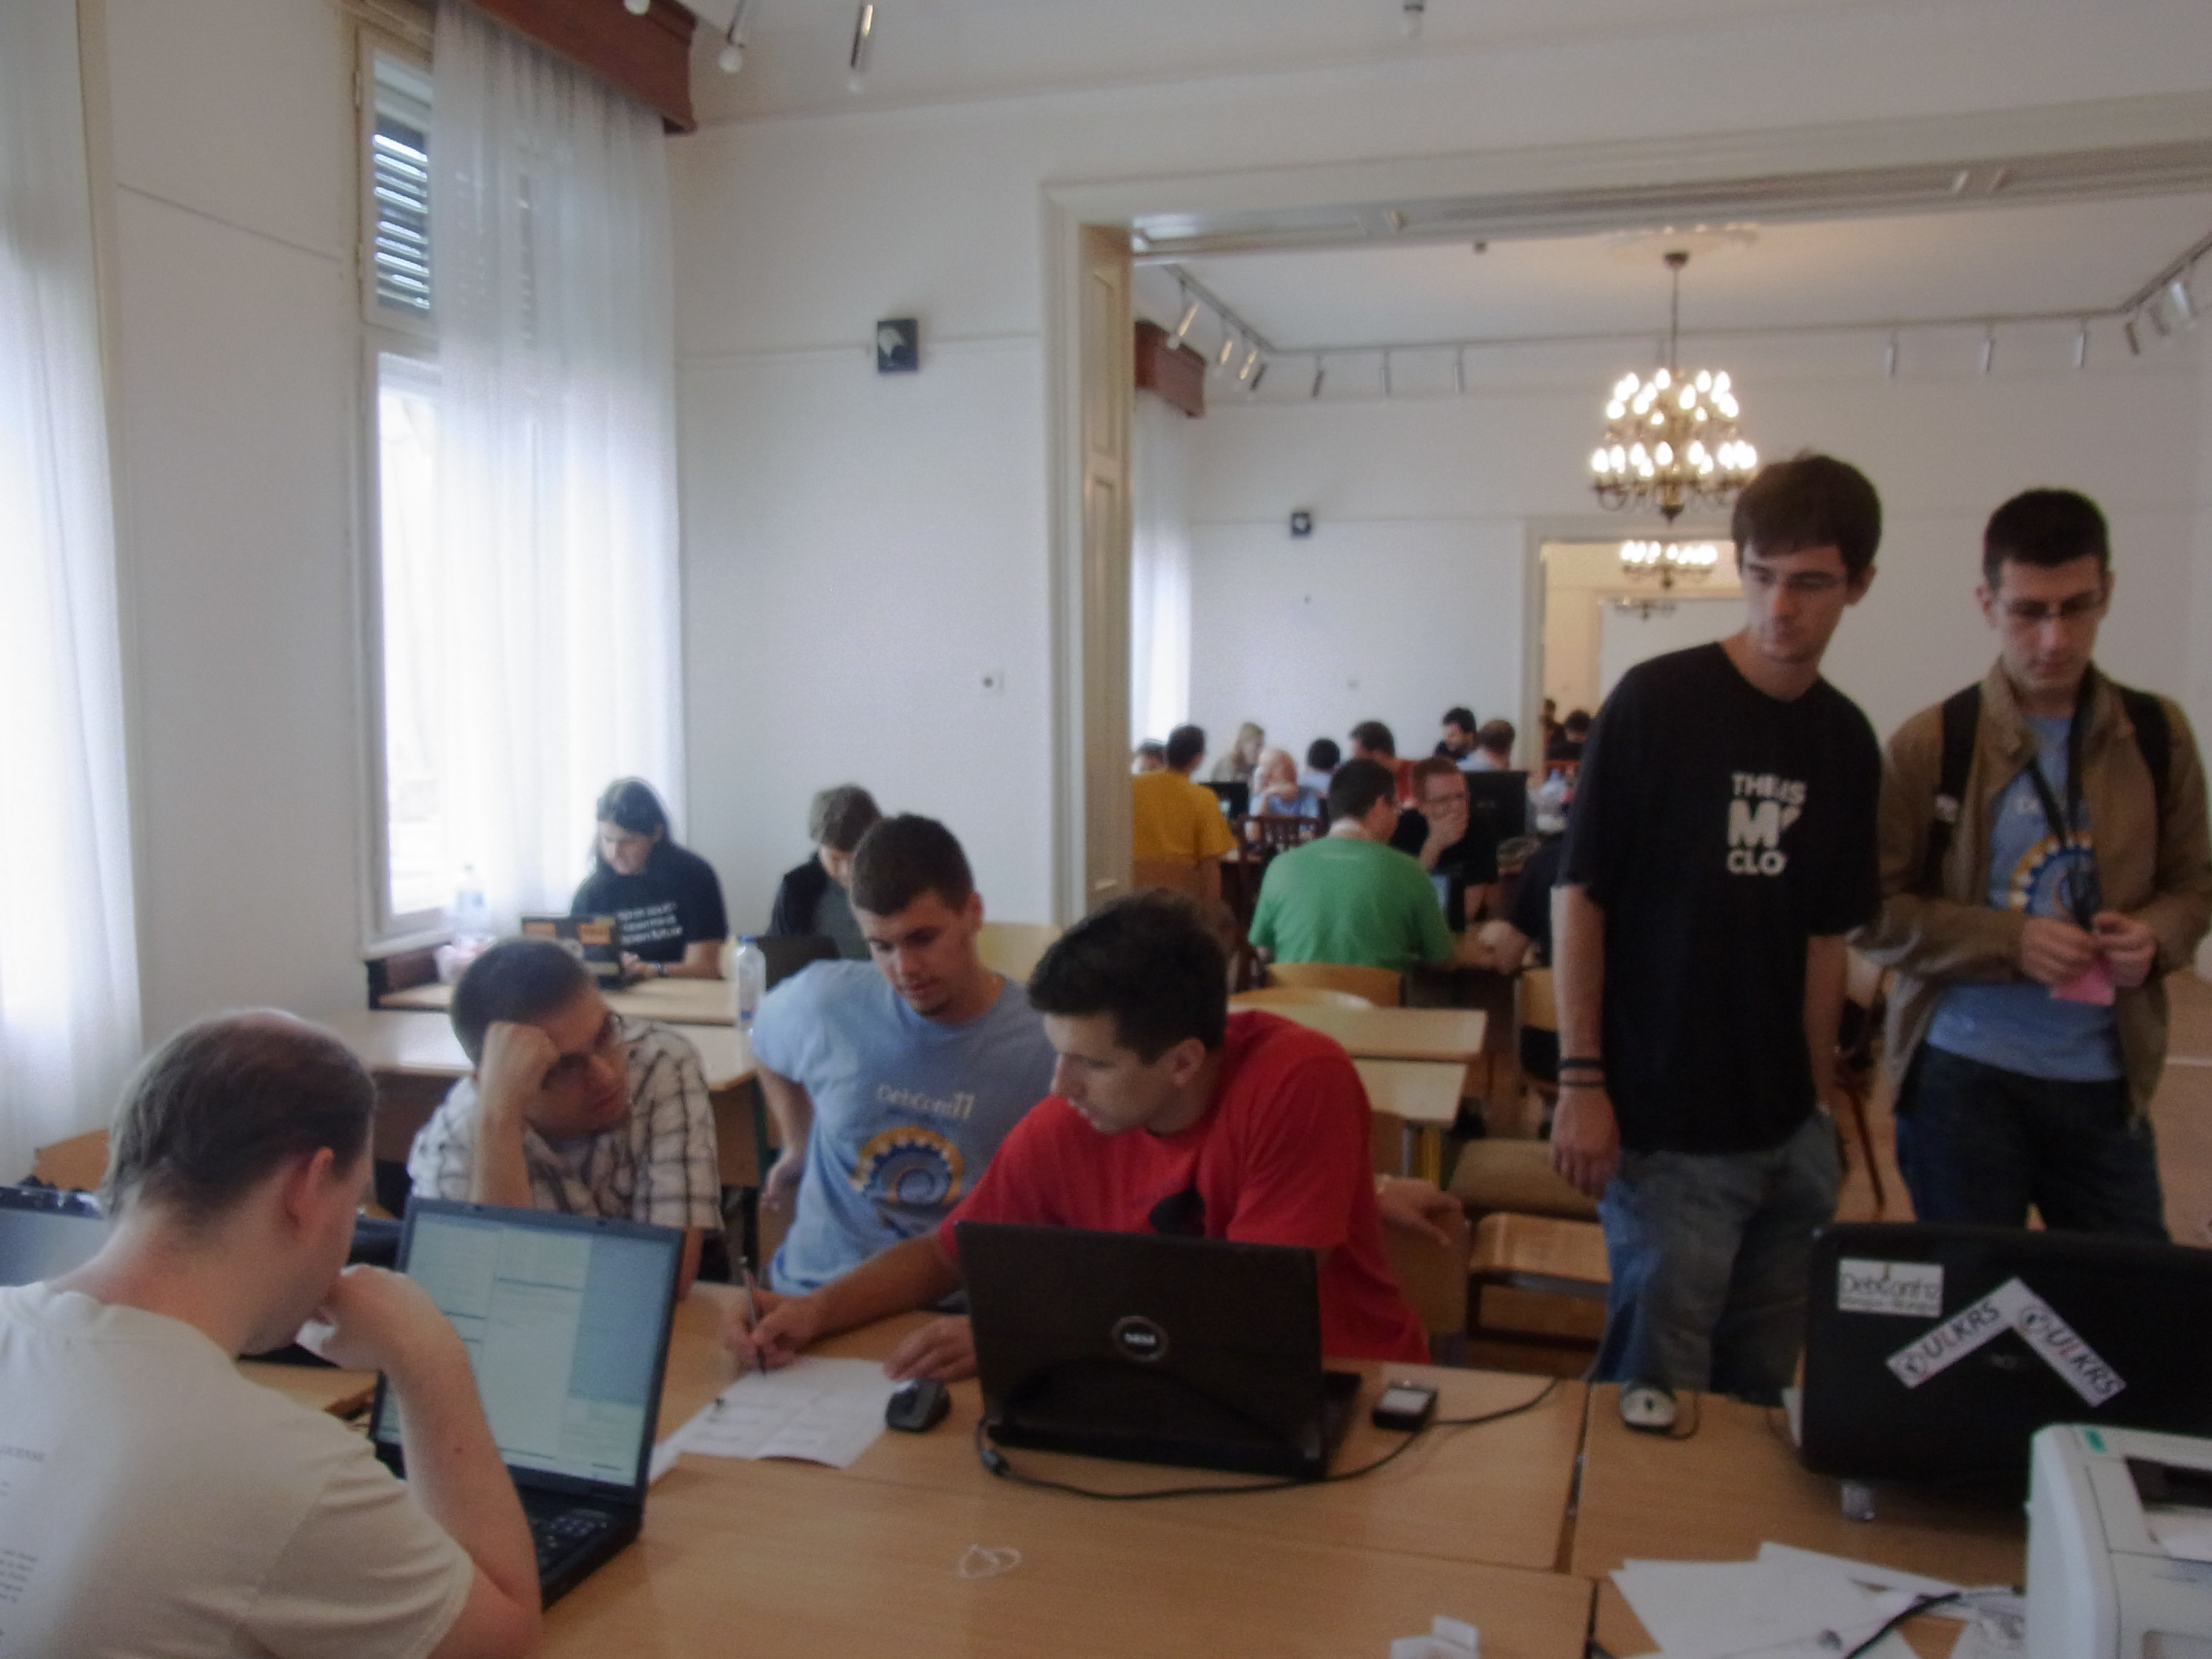
\includegraphics[width=0.9\hsize]{image201108/debconf11_hacklab2.jpg}
\end{center}
\end{frame}


\begin{frame}{GPGキーサインパーティ}
毎年恒例のGPG キーサインパーティ
\begin{center}
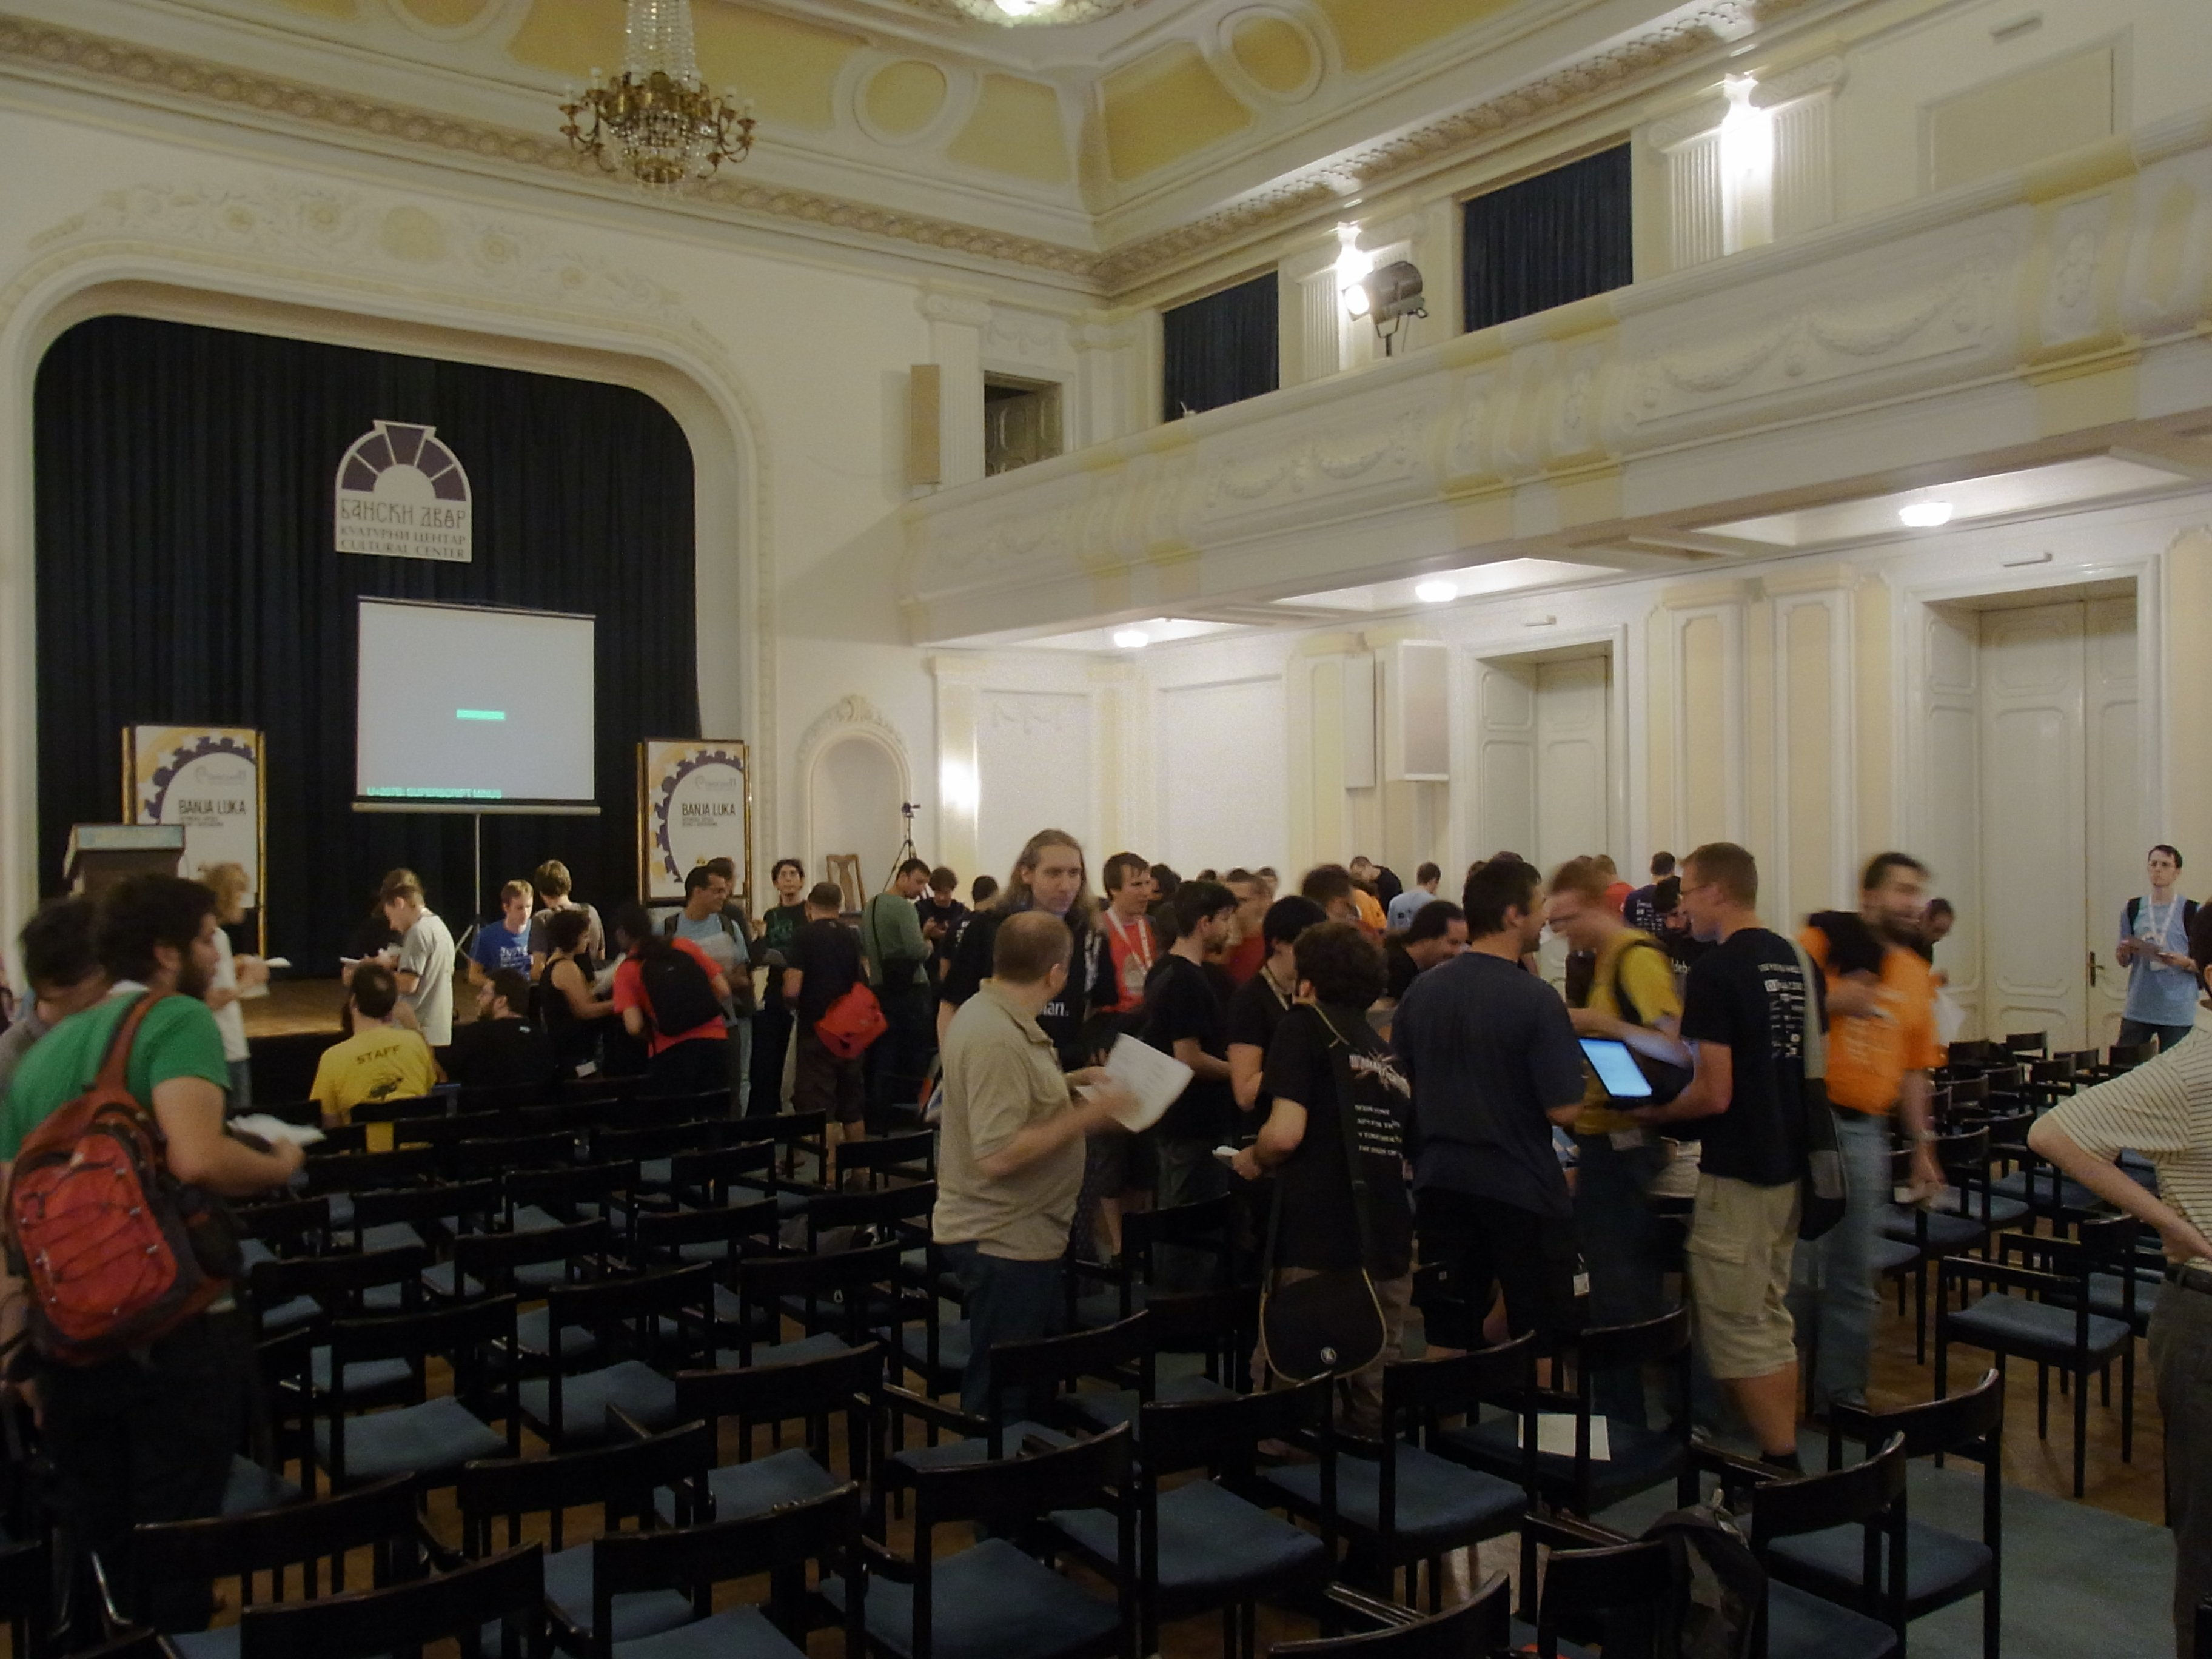
\includegraphics[width=0.9\hsize]{image201108/debconf11_ksp.jpg}
\end{center}
\end{frame}


\begin{frame}{チーズ\&ワインパーティ}
\begin{center}
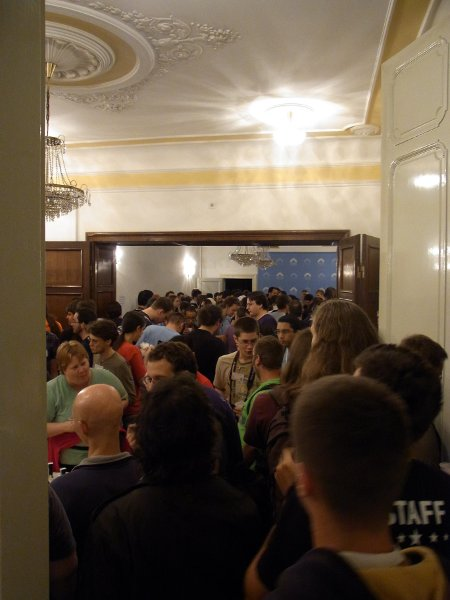
\includegraphics[height=0.9\hsize]{image201108/debconf11_cw.jpg}
\end{center}
\end{frame}



\begin{frame}{スケジュール}

24日のDebian Day で Debian Conference は開幕し、30日まで毎日いろいろな予
定が組まれた。
27日だけはカンファレンス参加者で Day Trip を実施した。

\end{frame}

\begin{frame}{主となった議論}

\begin{itemize}
\item multiarch のサポート
\item クロスコンパイルパッケージのサポート体制をどうするかの議論
\item Debian ブートストラップシステムについて
\item FTP master チームによる New queue 0
\item Test 駆動型開発をDebian やるには?(DEP8)
\item Linux kernel in Debian.
\end{itemize}

その他、Skill Exchange ということで、ハンズオンが多く行われた。
内容はパッケージング、git、Emacs の使い方など。

\end{frame}


\begin{frame}{次回のDebconf}

次回のDebconfは北米のマナグア/ニカラグアで開催される。
日本からはロサンゼルス経由で約15万円ほど。ビザは必要なし。

\end{frame}



\emtext{今後のイベント}
\begin{frame}{今後のイベント}
 
\begin{itemize}
 \item 9月 Debian温泉 2011、Debian 勉強会?
 \item 10月 Debian 勉強会 in 筑波大学、TeXユーザの集い2011(2011/10/22)
 \item 11月 OSC 2011 Tokyo/Fall 
\end{itemize}
\end{frame}

\begin{frame}{今日の宴会場所}

荻窪のどこか。
\end{frame}

\end{document}

;;; Local Variables: ***
;;; outline-regexp: "\\([ 	]*\\\\\\(documentstyle\\|documentclass\\|emtext\\|section\\|begin{frame}\\)\\*?[ 	]*[[{]\\|[]+\\)" ***
;;; End: ***
